\documentclass[12pt, a4paper]{article} % 10pt font size (11 and 12 also possible), A4 paper (letterpaper for US letter) and two column layout (remove for one column)

%----------------------------------------------------------------------------------------
%	PACKAGES AND OTHER DOCUMENT CONFIGURATIONS
%----------------------------------------------------------------------------------------

\usepackage[ngerman]{babel}

\usepackage[hang,small,labelfont=bf,up,textfont=it]{caption} % Custom captions under/above tables and figures

\usepackage{booktabs} % Horizontal rules in tables

\usepackage{graphicx} % Required for adding images
\graphicspath{{figure/}}

\usepackage{enumitem} % Required for customising lists
\setlist{noitemsep} % Remove spacing between bullet/numbered list elements

\usepackage[hidelinks]{hyperref}

\usepackage{tabularx}

\usepackage[verbose]{placeins}

\usepackage[official]{eurosym}

\usepackage{longtable}

\urlstyle{same}

\pretolerance=8000
\tolerance=5000
\emergencystretch=10pt % https://tex.stackexchange.com/questions/31301/how-to-reduce-the-number-of-hyphenation
\usepackage{indentfirst}

\usepackage[autostyle=true]{csquotes} % Required to generate language-dependent quotes in the bibliography

%----------------------------------------------------------------------------------------
%	MARGINS AND SPACING
%----------------------------------------------------------------------------------------

\usepackage{geometry} % Required for adjusting page dimensions
\usepackage{changepage}
\usepackage{calc}

\geometry{
    head=1cm,
    foot=3cm,
    top=2cm, % Top margin
    bottom=0cm, % Bottom margin
    left=3cm, % Left margin
    right=3cm, % Right margin
    includehead, % Include space for a header
    includefoot, % Include space for a footer
    %showframe, % Uncomment to show how the type block is set on the page
}

\setlength{\columnsep}{7mm} % Column separation width

%----------------------------------------------------------------------------------------
%	FONTS
%----------------------------------------------------------------------------------------

\usepackage[utf8]{inputenc} % Required for inputting international characters
\usepackage[T1]{fontenc}
\usepackage[default,scale=0.95]{opensans}
\usepackage{eurosym}

%----------------------------------------------------------------------------------------
%   TOC
%----------------------------------------------------------------------------------------
\setcounter{tocdepth}{2}

%----------------------------------------------------------------------------------------
%	HEADERS AND FOOTERS
%----------------------------------------------------------------------------------------

\usepackage{fancyhdr} % Needed to define custom headers/footers
\pagestyle{fancy} % Enables the custom headers/footers

\lhead{} % Left header

%----------------------------------------------------------------------------------------
%	TITLE SECTION
%----------------------------------------------------------------------------------------

\usepackage{titling} % Allows custom title configuration

\newcommand{\HorRule}{\rule{\linewidth}{1pt}} % Defines the horizontal rule around the title

\pretitle{
    \vspace{60pt} % Move the entire title section up
    \hspace{310pt}
    \\
    \\
    \vspace{40pt}
    \HorRule\vspace{10pt} % Horizontal rule before the title
    \centering\Huge\textbf
}

\posttitle{\par\vskip 15pt} % Whitespace under the title

\preauthor{} % Anything that will appear before \author is printed

\postauthor{ % Anything that will appear after \author is printed
    \vspace{10pt} % Space before the rule
    \par\HorRule % Horizontal rule after the title
    \vspace{150pt} % Space after the title section
}

\usepackage{xcolor}
\definecolor{df}{HTML}{b5dc17}
\usepackage{tikz}

\usepackage{eso-pic}
\newcommand\BackgroundPic{%
    \put(0,0){%
        \parbox[b][\paperheight]{\paperwidth}{%
            
\includegraphics[width=\paperwidth,height=\paperheight,keepaspectratio]{title_background.pdf}%
        }
    }
}


\fancyfootoffset[L]{\dimexpr\oddsidemargin+1in\relax}
\newcommand*\rect[1]{\begin{tikzpicture}[remember picture,overlay]\fill[df] (0,0) rectangle
        (\paperwidth,\headheight);\node at (0,0.5) {#1};\end{tikzpicture}}

\fancyfoot[L]{\rect{}}
\fancyfoot[C]{\rect{}}
\fancyfoot[R]{\rect{\thepage}}

 % Specifies the document structure and loads requires packages

\renewcommand\thepart{\Alph{part}}

%----------------------------------------------------------------------------------------
%	ARTICLE INFORMATION
%----------------------------------------------------------------------------------------

\begin{document}

\title{
Tür an Tür - Digital Factory gGmbH\\
Wirkungsbericht 2019\\
} % The article title

\AddToShipoutPicture*{\BackgroundPic}

\date{}

\maketitle
\thispagestyle{empty} % Disables header on first page (must be after \maketitle)

%----------------------------------------------------------------------------------------
%	ABSTRACT
%----------------------------------------------------------------------------------------

%----------------------------------------------------------------------------------------
%	ARTICLE CONTENTS
%----------------------------------------------------------------------------------------

\newpage
\tableofcontents

\newpage

\hypertarget{vorwort}{%
\section{Vorwort}\label{vorwort}}

Lieber Förderer, liebe Partner, liebe Wegbegleiterinnen und Wegbegleiter
von Integreat und der Tür an Tür - Digitalfabrik,

das Jahr 2019 war ein erfolgreiches und spannendes Jahr für unsere
Organisation und unsere Integrations-Plattform Integreat. Mit jedem Jahr
seit dem Bestehen der Tür an Tür - Digitalfabrik entwickeln wir uns
weiter. So sind wir zu einem beständigen und verlässlichen Partner für
öffentliche Stellen und soziale Projekte geworden, die wir durch
quelloffene IT-Lösungen bei der Erreichung ihrer jeweiligen
gemeinwohlorientierten Ziele unterstützen. In unseren Wirkungsberichten
dokumentieren wir jährlich unsere Fortschritte, Erkenntnisse und die
Rückmeldungen, die wir von unseren Partnern bekommen. Insbesondere in
Bezug auf die Integrations-Plattform Integreat, die seit 2015 in ganz
unterschiedlichen Städten und Landkreisen mit verschiedenem Fokus
eingesetzt wird, konnten wir in den letzten Jahren immer mehr
Möglichkeiten finden, die Wirkung des Projektes zu beobachten.

Den Eindrücken unserer kommunalen Partner kommt dabei eine entscheidende
Rolle zu und wir möchten in unserem diesjährigen Bericht diesen Stimmen
mehr Raum geben. So hat sich zum Beispiel erneut in kommunalen
Befragungen gezeigt, dass Integreat als fester Bestandteil von lokalen
Integrationsstrategien eingeplant wird. Die leichte Anpassbarkeit von
Inhalten, die Möglichkeit zur Informationsvermittlung an verschiedene
Zielgruppen und der Wissensaustausch mit anderen Kommunen
deutschlandweit überzeugen immer mehr Städte und Landkreise von der
Zusammenarbeit mit unserem Augsburger Sozialunternehmen Tür an Tür -
Digitalfabrik.

Unsere Erfahrungen aus der Skalierung der Integreat-Plattform helfen uns
auch dabei, neue Projekte in Angriff zu nehmen und von Anfang die
richtigen Fragen zu stellen. Nicht immer muss dabei das Rad neu erfunden
werden und häufig existieren bereits Lösungen, die durch Anpassungen für
neue Anwendungsfelder zugänglich gemacht werden können. Wir sind
gespannt auf die Entwicklungen, die sich daraus in den kommenden Jahren
ergeben werden und freuen uns auf ein erfolgreiches und vor allem
wirkungsvolles Jahr 2019 zurückblicken zu können.

In diesem Sinne wünschen wir viel Freude bei der Lektüre,


\includegraphics[width=2.03896in]{figure/Unterschrift_clara.jpg}

Clara Bracklo\\
Wirkungsmessung \& Organisationsentwicklung

\hypertarget{einleitung}{%
\section{Einleitung}\label{einleitung}}

\hypertarget{vision-und-ansatz}{%
\subsection{Vision und Ansatz}\label{vision-und-ansatz}}

Die Tür an Tür - Digitalfabrik gGmbH wurde im Juni 2016 mit dem Ziel
gegründet, Geflüchteten den Einstieg in ein neues gesellschaftliches
Leben zu erleichtern. Dieses Vorhaben wurde von Beginn an in
Zusammenarbeit mit etablierten und erfahrenen Organisationen und
Institutionen sowie kommunalen Verwaltungen verfolgt. Das starke
Netzwerk, das die Digitalfabrik seit den Anfängen des Projekts Integreat
im Jahr 2015 begleitet, ist seitdem wichtigste Voraussetzung für die
sich entfaltende Wirkung der Organisation.

Netzwerke aufzubauen und Synergiepotentiale zu identifizieren und
nutzbar zu machen, sind zum elementaren Teil der organisationalen Arbeit
geworden. Insbesondere in der intrakommunalen und interkommunalen
Zusammenarbeit konnten bereits Erfolge festgestellt werden. Unter
intrakommunaler Zusammenarbeit verstehen wir die Zusammenarbeit von
Akteuren innerhalb einer Kommune und unter interkommunaler
Zusammenarbeit die kommunenübergreifende Kollaboration und den damit
verbundenen Austausch. Auch weiterhin wollen wir dazu beitragen, dass
die Netzwerke in diesen beiden Bereichen gestärkt werden und die
vorhandenen Ressourcen in der Integrationsarbeit somit effektiv
eingesetzt werden können.

Die Vision, die wir mit unserer Arbeit verfolgen und deren
Verwirklichung als Maßstab für alle Aktivitäten der Organisation
auftritt, ist es, Informationen für alle Menschen verständlich und
barrierearm zugänglich zu machen. Die Marginalisierung von Menschen aus
anderen Ländern und Kulturen in der Gesellschaft ist oft auf
Informationsarmut begründet. Der Abbau von Informationsarmut durch
Lösungen wie Integreat und die damit gewonnene Gleichberechtigung im
Informationszugang stellen wichtige Meilensteine für die Entwicklung zu
einer freien und offenen Gesellschaft dar. Langfristig sind unsere
Angebote – insbesondere die Informations-App Integreat – darauf
ausgelegt, nicht nur Geflüchtete bei der Orientierung und
Informationsgewinnung zu unterstützen, sondern für alle Neuzugewanderten
und Bürgerinnen und Bürger als hilfreiche Stütze im Alltag und als
Kommunikationskanal der lokalen Verwaltung zu dienen. Wie der Name
bereits impliziert, will die Digitalfabrik digitale Brücken bauen, um
die lokale Integrationsarbeit zu stärken, ohne die persönliche
Beratungsstrukturen vor Ort ersetzen zu wollen.

Um diesen Fortschritt zu unterstützen und gleichzeitig das übergeordnete
Ziel von gemeinschaftlicher Entwicklung und Nutzung von Inhalten und
Software zu verfolgen, setzen wir in unserer Arbeit auf Open
Source-Technologien und verwenden Creative Commons-Lizenzen. So senken
wir Hemmschwellen und technische Barrieren, um die oben beschriebene
Zusammenarbeit initial zu befähigen, zu stärken und langfristig zu
etablieren. Frei nach dem Ansatz „Learning by Doing“ werden öffentliche
Verwaltungen durch Ansätze von uns an die Vorteile und Chancen, die
offen verfügbare Inhalte und Software bieten, herangeführt und können
diese in der eigenen Arbeit direkt erfahren. So können Erfolge der
Arbeit mit gemeinschaftlich erarbeiteter und offener Software und
Inhalten unter freier Lizenz in einem Bereich der Verwaltung – in diesem
Fall der Integrationsarbeit – verzeichnet werden. Daraus können wiederum
Transfermodelle und die Übernahme von Ansätzen und Methoden auch in
andere Bereiche innerhalb der Kommune entstehen. Wenn öffentliche Gelder
in die Entwicklung von Software oder von Inhalten investiert werden,
sollten diese auch der Öffentlichkeit zur Verfügung stehen. Davon sind
wir überzeugt und wollen mit unserer Arbeit gezielt zu dem
entsprechenden Systemwandel beitragen.

\hypertarget{gegenstand-dieses-berichts}{%
\subsection{Gegenstand dieses Berichts}\label{gegenstand-dieses-berichts}}

\noindent\begin{tabularx}{\textwidth}{p{4cm}X}
  \toprule
  Geltungsbereich & Dieser Bericht bezieht sich auf die Aktivitäten der
  Tür an Tür - Digital Factory gGmbH. Ein besonderer Fokus wird auf das
  zentrale Angebot von Integreat gelegt.\tabularnewline
  \midrule
  Berichtzeitraum und Berichtzyklus & Wir berichten über unsere Arbeit im
  Jahr 2019. Die Digitalfabrik veröffentlicht einmal im Jahr einen
  Wirkungsbericht.\tabularnewline
  \midrule
  Anwendung des SRS & In diesem Bericht orientieren wir uns an den
  Vorgaben der aktuellen Version des Social Reporting Standards (SRS),
  Stand 2014. Dies ist der dritte Jahresbericht nach dem
  SRS.\tabularnewline
  \midrule
  Ansprechpartnerin & \begin{minipage}[t]{\columnwidth}
  Clara Bracklo
  
  bracklo@integreat-app.de\end{minipage}\tabularnewline
  
  \bottomrule
\end{tabularx}

\hypertarget{die-gesellschaftliche-herausforderung-und-unser-luxf6sungsansatz}{%
\section{Die gesellschaftliche Herausforderung und unser
Lösungsansatz}\label{die-gesellschaftliche-herausforderung-und-unser-luxf6sungsansatz}}

\hypertarget{die-gesellschaftliche-herausforderung}{%
\subsection{Die gesellschaftliche
Herausforderung}\label{die-gesellschaftliche-herausforderung}}

Nach aktuellen Statistiken des UNHCR sind über 70 Millionen Menschen
derzeit weltweit auf der Flucht. Schätzungen zufolge suchen 41,3
Millionen von ihnen als Binnenflüchtlinge Schutz im eigenen Land. Einem
Großteil wurde allerdings durch Kriege und Verfolgung die Sicherheit in
der Heimat genommen und diese Menschen sind gezwungen das Heimatland zu
verlassen und in einem fremden Land Schutz zu suchen. Die
Herausforderungen, die sich dadurch für Organisationen, Länder und
Kommunen ergeben, sind auch in Europa und in Deutschland zu spüren.

Neben Flucht nimmt auch der Zuzug von Fachkräften aus dem Ausland eine
immer wichtigere Rolle in der Gestaltung von Integrationsprozessen ein.
Häufig suchen Akteure nach Möglichkeiten, um Angebote für eine größere
Zielgruppe zu schaffen. Dabei wird immer wieder deutlich, dass sich die
Herausforderung für das Ankommen und Leben in einer neuen Umgebung
unabhängig von dem Migrationshintergrund ähneln.

Zuwanderung stellt keine neue Entwicklung in Deutschland dar. Im
Vergleich zu früheren Migrationsbewegungen nach Deutschland, spielen
digitale Technologien für die Neuzugewanderten jedoch heute eine weitaus
bedeutendere Rolle, wie wir es auch in anderen Bereichen beobachten
können. Der Gebrauch von Smartphones zur Informationsbeschaffung ist
quer durch die Gesellschaft nahezu unabhängig von Altersstruktur und
kulturellem Hintergrund üblich. Auf der Flucht dient das Smartphone der
Kontaktaufnahme mit der Familie, als Navigator und der generellen
Informationsbeschaffung. Nach der Ankunft wird das Smartphone zur
Orientierung und als Kommunikationskanal genutzt und ist als wichtiges
Medium zur Integration zu verstehen. Auch Fachkräfte nutzen digitale
Informationszugänge, um sich vorab über potentielle Wohn- bzw.
Arbeitsorte zu informieren. Diesen Zugang jedoch effektiv zu nutzen
sowie Informationsangebote und Vernetzung anzubieten, ist insbesondere
für kommunale Verwaltungen, die bereits mit bestehenden Aufgaben stark
ausgelastet sind, nahezu unmöglich. Gemeinsame digitale
Kommunikationsräume existieren nicht. Selbst die Erstellung und
Aktualisierung mehrsprachiger Information stellt für viele Verwaltungen
eine große Herausforderung dar. Einen gemeinsamen Kommunikationsraum zu
schaffen, der die Verwaltungen, Organisationen und Neuzugewanderten
gleichermaßen zielgruppengerecht erreicht ist daher besonders wichtig,
um die Integrationsarbeit vor Ort langfristig zu verbessern und nach
Möglichkeit zu entlasten.

Über die letzten vier Jahre, in denen die Digitalfabrik im Bereich der
Integrationsarbeit tätig ist, konnten wir auf kommunaler Ebene ein
wachsendes Bewusstsein für die Bedarfe an Informationen und
Kommunikation verschiedener Migrantinnen- und Migrantengruppen –
insbesondere aus anderen europäischen Ländern – feststellen. Rechnet man
alle Migrationsbewegungen in ein neues europäisches Land zusammen,
ergibt sich eine Zahl von bis zu 4,9 Millionen Menschen im Jahr 2015.
Diese Zahl ist in den letzten zehn Jahren nicht ein einziges Mal unter
3,3 Millionen Menschen gefallen und zeigt die Bewegung innerhalb
Europas.

Dass Hilfsangebote sich nicht nur an einzelne Gruppen aus der
tagespolitischen Diskussion richten sollten und dürfen, ist ein
Anliegen, das die Digitalfabrik und ihre kommunalen Partner teilen.
Integrationsangebote für möglichst viele migrantische Zielgruppen und
kontextbezogene Akteure zugänglich zu machen, sichert die
Langfristigkeit der Projekte und kann die Wirkung der Aktivitäten
ausweiten und verstärken.

Neben den wichtigen gesellschaftlichen Entwicklungen aus dem Bereich der
Integration und Zuwanderung ist abschließend die aktuelle öffentliche
Debatte zur Verwendung und Entwicklung freier und quelloffener Software
(Open Source Software) in der Verwaltung zu nennen. Die Forderung
verschiedener Organisationen lässt sich folgendermaßen zusammenfassen:
Werden öffentliche Gelder (Steuergelder) zur Entwicklung oder Nutzung
von Software eingesetzt, so soll die Software selbst ebenfalls
öffentlich und frei zugänglich sein und nicht von einzelnen Unternehmen
unter Verschluss gehalten werden. Der Systemwandel, der zur
Verwirklichung dieser Forderung notwendig ist, ist komplex und muss alte
Strukturen aufbrechen. Die damit einhergehende Herausforderung ist somit
nicht zu unterschätzen.

\hypertarget{die-angebotslandschaft}{%
\subsection{Die Angebotslandschaft}\label{die-angebotslandschaft}}

Der soziale Bereich bietet viele unerschlossene Potentiale für digitale
Lösungen, die Prozesse vereinfachen, Menschen vernetzen und Wissen für
jeden zugänglich machen können. Die Digitalfabrik konzentriert sich in
erster Linie auf den Bereich Integration.

Neben der persönlichen Beratung, die unserer Meinung nach aufgrund der
heterogenen und individuellen Sachverhalte immer zentraler Bestandteil
des Integrationsprozesses sein sollte und sein muss, haben Kommunen die
Bekanntmachung von lokalen Informationen und Angeboten in der
Vergangenheit vor allem durch das Verfassen und aufwendige Drucken sowie
Verteilen von Printmaterialien forciert. Waren die Printmaterialien
einmal gedruckt, ließen sich die Inhalte nur mit großer zeitlicher
Verzögerung und viel Aufwand aktualisieren. Entsprechendes
Informationsmaterial von Verwaltungen war häufig nur in deutscher
Sprache verfügbar, da Übersetzungen nicht nur teuer, sondern auch
aufwendig herzustellen waren.

Digitale Technologien stellen einen geeigneten Weg zur Vermittlung von
Informationen an neuzugewanderte Menschen dar, da Mehrsprachigkeit
leichter und kostengünstiger umsetzbar und neue Informationen einfach
über den bestehenden digitalen Kanal ohne zeitlichen Verzug
weitergegeben werden können. Somit bieten entsprechende Technologien
eine leicht aktualisierbare und gut zugängliche Alternative zu
herkömmlichen Printmaterialien. Diese Erkenntnis motivierte verschiedene
etablierte und auch neue Unternehmen und Organisationen zur Entwicklung
von digitalen Lösungen.

In der Gründungszeit der Digitalfabrik Mitte 2016 entstanden somit neben
der hauseigenen Informations-App Integreat auch andere
Informationsportale von verschiedenen Anbietern. Zu nennen sind an
dieser Stelle unter anderem die Ankommen-App des BAMF, die App Moin
Refugee, die Welcome App Germany und die App Welcome to NRW als Angebote
in Deutschland. Gemeinsam ist diesen Angeboten und der
Integreat-Plattform die grundsätzliche Darstellung von Informationen für
Neuzugewanderte. Trotz bestimmter Überschneidungen ist über zwei Jahre
nach der besonders starken Zuwanderung 2015 auffällig, dass die Angebote
mit Ausnahme der Integreat-Plattform nur noch partiell oder gar nicht
mehr weiterentwickelt werden.

\hypertarget{die-projekte-der-tuxfcr-an-tuxfcr-digitalfabrik-ggmbh}{%
\subsection{Die Projekte der Tür an Tür – Digitalfabrik
gGmbH}\label{die-projekte-der-tuxfcr-an-tuxfcr-digitalfabrik-ggmbh}}

Um dieses Phänomen zu verstehen und gleichzeitig an die Wirkung der
Digitalfabrik heranzuführen, ist die Positionierung der Organisation in
dieser Angebotslandschaft besonders relevant. Bereits die
Entstehungsgeschichte der Organisation ist für den besonderen Charakter
beschreibend. So wurde die Organisation nicht um ihrer selbst wegen
gegründet, sondern war Ergebnis von organischem, bedarfsorientiertem
Wachstum.

Als im Jahr 2015 über eine Million Geflüchtete nach Deutschland kamen,
wurde der Bedarf an mehrsprachigen Informationsangeboten zu Asylthemen
und Alltagsfragen schnell deutlich. In Augsburg arbeiteten der Verein
Tür an Tür - miteinander wohnen und leben e.V. (Tür an Tür e.V.), die
Stadt Augsburg und der Lehrstuhl für Wirtschaftsinformatik der TU
München gemeinsam an der Digitalisierung der 1997 erschienenen „First
Steps“-Broschüre mit lokalen Erstinformationen für Asylbewerberinnen und
Asylbewerber in der Region Augsburg. Als Ergebnis entstand im Sommer
2015 die Integreat-Plattform (ehemals RefGuide+) als digitaler
Alltagsguide für Geflüchtete, die in Augsburg im November 2015 offiziell
von allen Projektpartnern vorgestellt wurde. Nach der Bekanntmachung der
Integreat-Plattform in und für Augsburg, zeigten auch weitere Städte und
Landkreise ihr Interesse daran, die Lösung in der eigenen Region
einzusetzen. Die Gründung der Tür an Tür – Digitalfabrik gGmbH folgte im
Sommer 2016 aufgrund der direkten Anfrage und dem Bedarf der kommunalen
Partner, die Zusammenarbeit an der Integreat-Plattform professionell zu
gestalten und für die Kommunen für Planungssicherheit zu sorgen.

Mittlerweile hat sich die Digitalfabrik zu einem Beratungs- und
Dienstleistungsunternehmen für verschiedene digitale Projekte im
sozialen und öffentlichen Bereich entwickelt. Die Erfahrungen und
Expertise, die durch die mehrjährige Zusammenarbeit mit Institutionen
aus beiden Bereichen gewonnen wurden, geben wir in unserer täglichen
Arbeit an unsere Partner und gleichgesinnte Organisationen weiter. Das
im Laufe dieser Zeit entstandene Netzwerk stellt eine wichtige Grundlage
für unsere Aktivitäten dar und ermöglicht es, Ressourcen gemeinsam zu
nutzen und im nächsten Schritt auch anderen zugänglich zu machen.

Die Digitalfabrik versteht sich als Wegbereiter für die positive
Entwicklung und Öffnung von öffentlichen und sozialen Institutionen
durch Einsatz digitaler Lösungen. Dies unterstützen wir mit all unseren
Aktivitäten. Aufgrund der besonderen Relevanz und des Einflusses auf die
wirkungsorientierte Arbeitsweise, soll im Folgenden die App Integreat
genauer vorgestellt werden.

\hypertarget{die-integrations-plattform-integreat}{%
\subsubsection{Die Integrations-Plattform
Integreat}\label{die-integrations-plattform-integreat}}

Das Herzstück der Digitalfabrik ist die Integrations-Plattform
Integreat. Dieses Angebot, welches ursprünglich für Geflüchtete
entwickelt wurde, richtet sich heute an eine breitere Zielgruppe. Im
Fokus stehen dabei Neuzugewanderte, die sich selbstständig in ihrer
neuen Region informieren möchten. Jede Kommune entscheidet dabei, welche
Zielgruppe (z.B. Geflüchtete, Ehrenamtliche, alle Migrantinnen und
Migranten) angesprochen wird.

Auf kommunaler Ebene ist der Bedarf an einem gemeinsamen
Kommunikationsraum für Beraterinnen und Berater, Verwaltung,
Ehrenamtliche und Neuzugewanderte besonders hoch. Die Kommunikation
findet meist bilateral zwischen den Neuzugewanderten als Einzelpersonen
und den verschiedenen Akteuren statt. Gleichzeitig befindet sich das
Wissen im Bereich Integration häufig in den Köpfen der Beraterinnen und
Berater und ist nur selten verschriftlicht und somit frei zugänglich.
Hier kann durch die gezielte Bündelung der Informationen an einer
zentralen und neutralen Stelle, der Integreat-Plattform, mehr
Transparenz für alle Akteure hergestellt werden. Durch diese Bündelung
erhöht sich nicht nur die Verständlichkeit von Prozessen für
Neuzugewanderte, sondern es entsteht auch eine transparente Angebots-
und Wissensdatenbank.

Um Kommunen ein konkretes Mittel an die Hand zu geben, um diese
Transparenz ohne große Kosten und technisches Know-how herstellen zu
können, wurde Integreat ins Leben gerufen: Für die Menschen, die durch
Flucht oder Migration in eine fremde Kultur kommen, stellt sich
Integreat in Form einer mobilen App dar. Für die Kommunen ist Integreat
eine Integrations-Plattform, auf der Informationen und lokale Angebote
verwaltet werden. Integreat ermöglicht den einfachen Informationsfluss
zwischen Kommunen, Hilfsorganisationen und Menschen mit Flucht- oder
Migrationshintergrund – egal ob in einer kleinen Gemeinde, einer Stadt
oder einem Landkreis.

Mit Integreat werden Menschen im Alltag wichtige Informationen in einer
kostenlosen und offline nutzbaren App zur Verfügung gestellt. Durch die
Mehrsprachigkeit werden Sprachbarrieren überwunden. Darüber hinaus
bildet Integreat langfristig ein digitales Fundament für weitere
kommunale Integrationsarbeit, schafft also durch eine zentrale Sammlung
von relevanten Prozessen, Angeboten und Kontakten in einer Kommune die
Grundlage für weitere Maßnahmen und Aktivitäten. Die Inhalte werden von
lokalen Institutionen und Initiativen unter kommunaler Verwaltung
gepflegt. Transparenz und gemeinwohlorientierte Entscheidungen sind die
Basis des Projekts.

Kern der Lösung ist eine mobile Applikation (Frontend) in Kombination
mit einem intuitiv zu bedienenden Informationsverwaltungssystem
(Backend). Entschließt sich eine Kommune oder ein anderer Träger für
Integreat, bekommen diese einen eigenen geschlossenen Bereich auf der
Integreat-Plattform, welcher auf Wunsch bereits eine deutschlandweit
gültige Vorlage in mehreren Sprachen enthält, die die Kommune dann um
lokale Informationen ergänzen kann. Ein weiteres Angebot ist die
integrierte Web-App mit Hilfe derer auch über eine Webseite oder
Suchmaschinen auf die mehrsprachigen Inhalte zugegriffen werden kann.
Der aktuelle Stand der Informationen kann jederzeit ausgedruckt werden
und so können auch diejenigen ohne Smartphone oder Computer erreicht
werden.

Im Gegensatz zu anderen Lösungen am Markt entfaltet Integreat die
Wirkung auf lokaler Ebene, ist gleichzeitig aber nahezu unbegrenzt
skalierbar. Die Lokalität der Informationen für Neuzugewanderte ist
deshalb so wichtig, da sich Prozesse und Zuständigkeiten von
Institutionen oft innerhalb desselben Bundeslandes, noch öfter aber im
Regierungsbezirk und Kommunalverwaltung unterscheiden. Die Genauigkeit
und Aktualität der Informationen werden gewährleistet, da die Inhalte
von hauptamtlichen Akteuren vor Ort eingestellt und gepflegt werden.
Voraussetzung für die Nutzung von Integreat als Kommunen ist die
Verfügbarkeit von mindestens einer hauptamtlichen Person, die das
Integreat-Projekt vor Ort koordiniert und Inhalte federführend
aktualisiert. Das Team von Integreat kann sich so auf seine Stärken, die
Weiterentwicklung von Plattform und App, die Suchmaschinenoptimierung,
die Vernetzung, die Einbindung neuer Funktionen und die Beratung der
Kommunen und Landkreise, konzentrieren.

Gestartet im November 2015 mit Augsburg als Pilotstadt, arbeiten Ende
2019 bereits 59 Kommunen und Kreise mit Integreat an einer verbesserten
Informationsversorgung für Neuzugewanderten vor Ort. Das Projekt
Integreat bietet Ehrenamtlichen in ganz Deutschland die Möglichkeit an
einem sozialen Open Source-Projekt zu arbeiten, ihre Fähigkeiten zu
erproben und als diversifiziertes Team zur verbesserten Integration in
unserer Gesellschaft beizutragen. Die Digitalfabrik bietet die
organisatorische Struktur, um den Mitarbeitenden im Projekt die nötige
Freiheit und Sicherheit zu gewährleisten. Langfristig sollen nach dem
Modell von Integreat weitere eigenständige Projekte entstehen und
gefördert werden.

\hypertarget{weitere-projekte}{%
\subsubsection{Weitere Projekte}\label{weitere-projekte}}

Alle Projekte, die in Zusammenarbeit mit der Digitalfabrik entstehen,
entwickeln sich aus einem konkreten Bedarf. Als Organisation unterstützt
die Digitalfabrik mit digitalen Angeboten im gemeinwohlorientierten
Bereich und trägt somit dazu bei, dass NPOs - d.h. Organisationen, die
keine gewinnorientierten Ziele verfolgen - und Initiativen ihre
wirkungsorientierten Ziele durch passende IT-Lösungen besser erreichen
können. Im Folgenden sollen die bisher umgesetzten Projekte in Kürze
vorgestellt werden.

\hypertarget{projekte-im-augsburger-raum}{%
\paragraph{\texorpdfstring{Projekte im Augsburger Raum
}{Projekte im Augsburger Raum }}\label{projekte-im-augsburger-raum}}

Angelehnt an den EDV-Führerschein in Nordrhein-Westfalen und andere
grundlegende Computerkurse haben wir uns gemeinsam mit Prof. Dr.
Wolfgang Klüver, ehemaliger Informatik-Professor an der Hochschule
Augsburg, Gedanken gemacht, wie ein derartiges Format für
neuzugewanderte Menschen aussehen kann. Mit fit for IT (kurz: ffIT)
haben wir eine Kursreihe ins Leben gerufen, die grundlegende
Fertigkeiten und Kenntnisse am Computer, Smartphone und im Umgang mit
dem Internet schult. Der ffIT-Kurs besteht aus 8 Kursstunden á 90
Minuten und wird im Café Tür an Tür in Augsburg durchgeführt. Der Kurs
schließt ebenfalls mit einem EDV-Führerschein ab. Das
Mindestsprachniveau für die Kursreihe liegt bei A2. Am Ende des Kurses
können die Teilnehmerinnen und Teilnehmer das Internet für Suchanfragen
verwenden, Kontakt aufnehmen (E-Mail), Bewerbungsunterlagen schreiben
und Wohnungen suchen.

Ein weiteres, ehrenamtlich getragenes und von der Digitalfabrik
betreutes Projekt im Augsburger Raum ist die Installation von
Internetzugängen in mehreren lokalen und gemeinschaftlichen Unterkünften
für Geflüchtete (kurz: WLAN-Projekt). Mit Eigenmitteln und Ehrenamt
wurden die initialen Investitionen zum Ausbau in den
Gemeinschaftsunterkünften für Geflüchtete in der Ottostraße,
Zusamstraße, im Mühlmahdweg sowie für Aussiedlerinnen und Aussiedler in
der Windprechtstraße in Augsburg vorgenommen. Der Internetzugang kann
gemeinschaftlich von allen Bewohnerinnen und Bewohnern genutzt werden.
Außerdem haben wir seit Ende 2019 auch den technischen Betrieb der
Schülestraße vom Verein Refugees Online e.V. übernommen. Der
Installations-, Wartungs- und Betreuungsaufwand wird von Ehrenamtlichen
aus unserem Netzwerk bewältigt. Der Zugang zum Internet für die nun bis
zu 600 versorgten Menschen hilft dabei, lokale Integrationsprozesse
fördern und vereinfachen. Mittlerweile gibt es immer mehr digitale
Angebote für Geflüchtete, sei es um zusätzlich zu den Deutschkursen, die
Sprache durch entsprechende Online-Angebote vertiefen zu können, sich
über das Leben und aktuelle Geschehen in Deutschland und Augsburg zu
informieren oder nach einem Arbeits- oder Praktikumsplatz zu suchen.

\hypertarget{kooperationsprojekte}{%
\paragraph{Kooperationsprojekte}\label{kooperationsprojekte}}

Zwei Projekte, die in der Vergangenheit umgesetzt wurden, aber aktuell
aufgrund fehlender Nachfrage nicht mehr aktiv weitergeführt werden, sind
das als modulare Willkommensmappe entworfene Arrival Kit und die zur
Angliederung an die App Integreat entwickelte Wohnraumbörse.

Das \textbf{Arrival Kit} ist ein hochwertiges digitales Print-Produkt.
Als modulare Willkommensmappe verbindet es fünf Elemente: Einen
Stadtplan inkl. Anlaufstellen und Behördenwegweiser, einen
Basiswortschatz in deutscher Sprache, eine ebenfalls mehrsprachige
Broschüre zum Asylverfahren, ein bebildertes Heft mit Tipps für den
Alltag, sowie die Mappe selbst, die gleichermaßen individualisiert
werden kann und z.B. Platz für ein Anschreiben/Willkommenstext bietet.
In Augsburg wurde das Arrival Kit in Zusammenarbeit mit der Stadt
Augsburg und dem netzwerk4A als Leuchtturmprojekt umgesetzt.

Gemeinsam mit zwei Gebietskörperschaften in Bayern wurde 2018 eine
digitale \textbf{Wohnraumbörse} nach dem “Passauer Modell” entwickelt.
Das Angebot richtet sich an potentielle Vermieterinnen und Vermieter,
die ihre Mietobjekte an Neuzugewanderte vergeben möchten. Das Projekt
wurde Open Source entwickelt und ist als freie Software verfügbar. Das
Projekt wurde über Mittel des bayerischen Sozialministeriums finanziert.
Es erfüllt die Kriterien und Funktionen, die das „Passauer Modell“
ebenfalls in sich vereint - stellt also einen digitalen Briefkasten für
Wohnungsangebote bereit -, arbeitet aber mit Webformularen und wurde in
Kombination mit der Integreat-Plattform vollautomatisiert betrieben.

\hypertarget{die-wirkung-der-digitalfabrik}{%
\section{Die Wirkung der
Digitalfabrik}\label{die-wirkung-der-digitalfabrik}}

\hypertarget{transparenz-durch-vernetzung-und-digitalisierung}{%
\subsection{Transparenz durch Vernetzung und
Digitalisierung}\label{transparenz-durch-vernetzung-und-digitalisierung}}

Die offene Gestaltung unserer Gesellschaft und die damit verbundene
erleichterte Integration von Neuzugewanderten sind komplexe
Herausforderungen, auf die keine einseitige Antwort durch eine einzelne
Institution gegeben werden kann. Unser Selbstverständnis als
Organisation beruht stark auf der Zusammenarbeit mit anderen Akteuren im
Netzwerk. Wir setzen uns mit unserer Arbeit dafür ein, unterschiedliche
Ressourcen im Bereich der Integrationsarbeit zu verbinden und nutzbar zu
machen. In der Vernetzung mit langjährig etablierten Institutionen aus
diesem Bereich und kommunalen Verwaltungen entstehen besondere
Synergiepotentiale, die durch die Digitalfabrik erschlossen werden. Wir
geben Expertise weiter, schaffen durch Informations- und
Technologietransparenz die Strukturen, um gemeinsame Inhalte und
Technologien nutzbar zu machen und auch über unsere Organisation zur
Verfügung zu stellen.

Um im Folgenden die Wirkung der einzelnen Aktivitäten darstellen zu
können, ist die differenzierte Betrachtung unserer wichtigsten Kunden
und Nutzerinnen- und Nutzergruppen notwendig. Unterschieden wird hier
zwischen den Neuzugewanderten als Nutzerinnen und Nutzer bzw.
Empfängerinnen und Empfänger der Angebote und den kommunalen
Verwaltungen als Kunden.

Gleichzeitig wirken alle Aktivitäten unabhängig von der direkten
Zielgruppe auf die gleichen mittel- und langfristigen Ziele ein. Diese
werden projektspezifisch in einer Wirkungslogik ausgearbeitet, sobald
ein Projekt sich nach der Pilotphase auch langfristig etabliert und die
Komplexität eine detaillierte Aufstellung erfordert. In diesem Bericht
wird daher lediglich eine detaillierte Aufstellung für das
Integreat-Projekt und die damit verbundenen Aktivitäten vorgenommen.

\hypertarget{unterstuxfctzung-von-neuzugewanderten}{%
\subsection{Unterstützung von
Neuzugewanderten}\label{unterstuxfctzung-von-neuzugewanderten}}

An erster Stelle in der strategischen Entwicklung und der Arbeit in den
einzelnen Projekten der Digitalfabrik stehen die Bedürfnisse von
zugewanderten Menschen in Deutschland. Ausdrücklich werden hierbei
Geflüchtete und Menschen, die gerade erst nach Deutschland gekommen sind
(Neuzugewanderte/Fachkräfte), miteingeschlossen.

Die Erweiterung beziehungsweise Öffnung der primären Zielgruppe für die
Angebote um Integreat wird besonders deutlich in der Außenkommunikation
für die Integreat-Plattform sowie den Herausforderungen, die durch
unsere kommunalen Partner geschildert werden. Während die
Integreat-Plattform zu Beginn als Angebot für „Asylsuchende“ deklariert
wurde, ging die Entwicklung über „Flüchtlinge“ zu „Geflüchteten“ über
„Menschen mit Migrations- und Fluchthintergrund“ hin zu dem aktuellen
Stand der „Neuzugewanderten“. Eine eindeutige Unterscheidung zwischen
Geflüchteten und anderen Migrantengruppen ist von Grund auf
problematisch – und für die Arbeit der Digitalfabrik nicht zwingend
notwendig – da die Fluchtsituation oftmals weitere Migrationsbewegungen
mit sich bringt. Dementsprechend gestalten wir unsere Angebote
heutzutage offen zur individuellen lokalen Gestaltung, um den
Herausforderungen vor Ort bestmöglich zu entsprechen. Die Veränderung
stellt sich also sichtbar im Namen dar, betrifft darunterliegend aber
vor allem in Inhalte, Sprachangebot und begleitenden Maßnahmen.
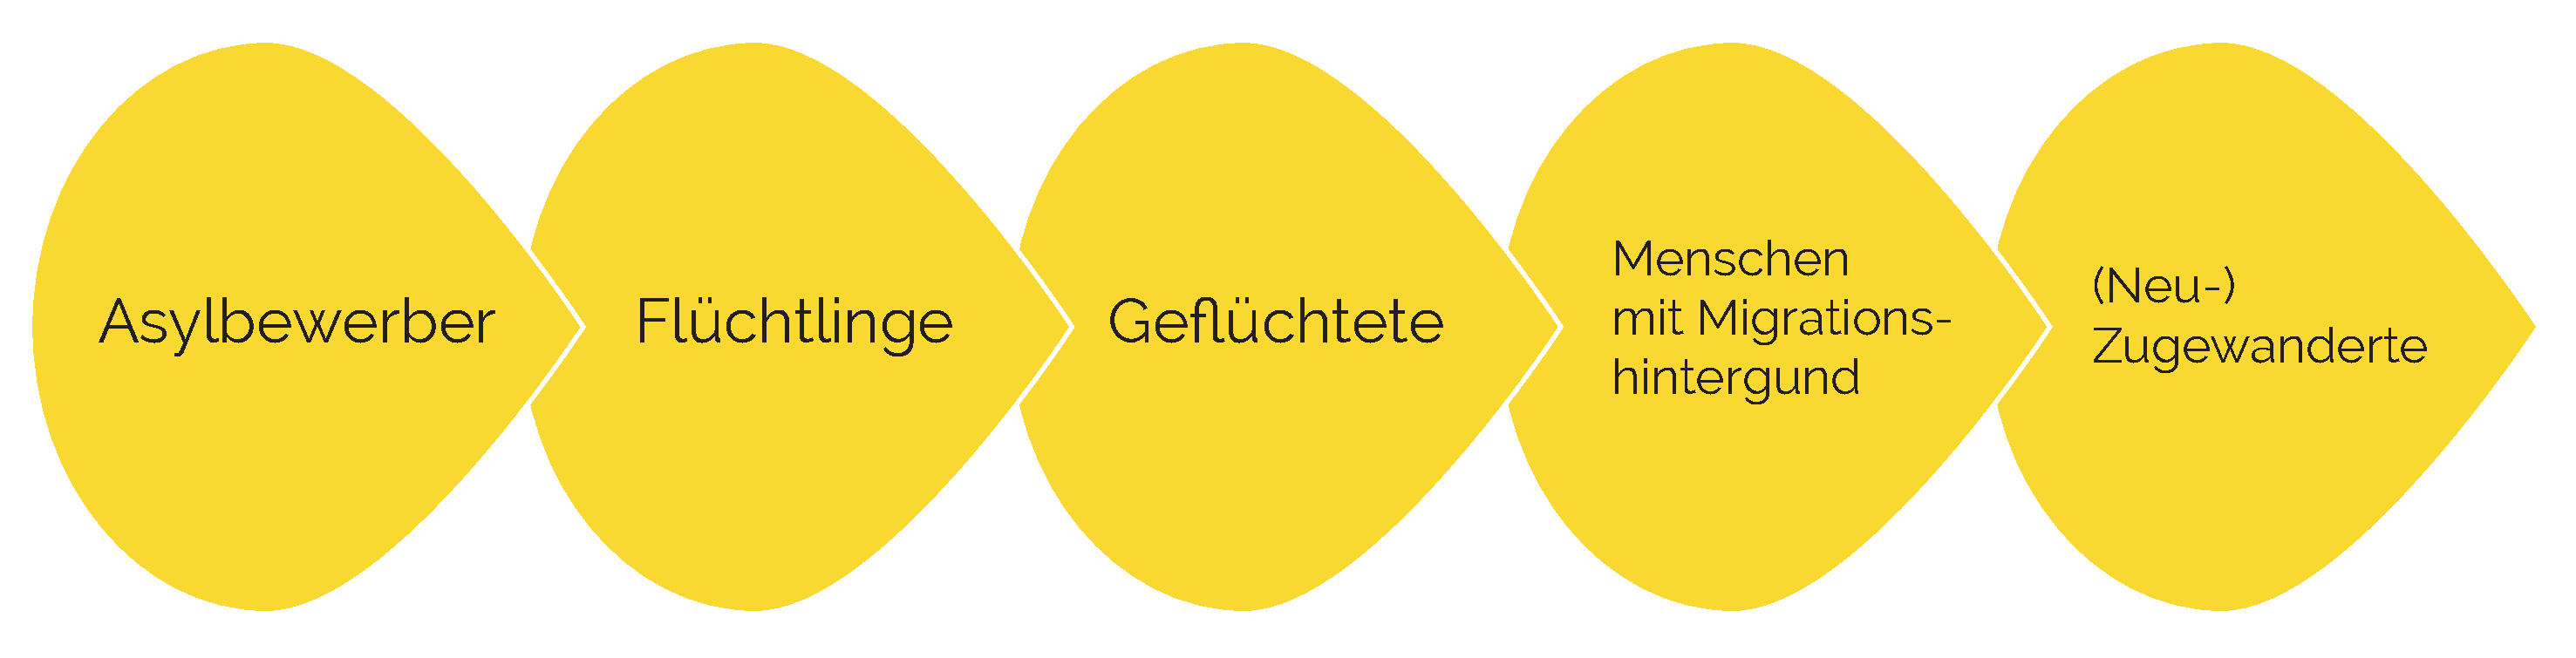
\includegraphics[width=\textwidth]{figure/Flowchart.pdf}

\hypertarget{leistungen-fuxfcr-neuzugewanderte}{%
\subsubsection{Leistungen für
Neuzugewanderte}\label{leistungen-fuxfcr-neuzugewanderte}}

Im Kontext von Integreat lag der Fokus im Jahr 2019 darauf, erste
Schritte zu unternehmen, um die Integreat-Technologie auch außerhalb
Deutschlands bekannt zu machen und somit den Wirkungsradius zu
vergrößern. bisher unerschlossene Benutzerinnen- und Benutzergruppen
ansprechen zu können. Hierfür musste zunächst sichergestellt werden,
dass die Integreat-Technologie auch ohne das direkte Zutun des
Digitalfabrik-Entwicklungsteams einsetzbar ist. Hintergrund ist die
eingeschränkte Skalierbarkeit, die durch die Grenzen unsere Organisation
bedingt ist, wenn wir versuchen die Wirkung nur direkt über unsere
eigenen Aktivitäten zu erzielen. Ziel muss es sein, die indirekte
Wirkung zu maximieren, also andere Organisationen zu befähigen mit
durich uns entwickelten Open Source-Technologien ihr eigenen analogen
Wirkungsziele zu erreichen. In diesem Kontext war vor allem die
Umstellung der Technologie auf React Native ein wichtiger Schritt, der
auch die Nachhaltigkeit des Projekts sicherstellt und 2020
fertiggestellt wird. Zudem ermöglichen die Aktivitäten des Jahres 2019
die Technologie auch unter anderem Branding für weitere Zielgruppen
einzusetzen. Um die Sichtbarkeit des Integreat-Projektes bzw. der
vielseitig einsetzbaren Technologie auch im internationalen Raum zu
fördern, wurden 2019 verschiedene Netzwerke und Kontakte zu
Organisationen und Initiativen in unterschiedlichen Ländern aufgebaut.

Besonders fruchtbar war hierbei der Austausch mit Akteuren in Sydney zum
Einsatz der Integreat-Technologie vor Ort und einem Projekt aus
Großbritannien, das sich für die Bildung junger geflüchteter Menschen in
der Türkei, in Uganda, Pakistan, Bangladesch, dem Libanon und Äthiopien
einsetzt.

2019 wurde außerdem durch die Einbettung einer standortbezogenen
Übersicht über Integreat-Kommunen in der Nähe eine technische
Erweiterung umgesetzt, die die Bedienbarkeit der Lösung erleichtert.

\hypertarget{intendierte-wirkungen}{%
\subsubsection{Intendierte
Wirkungen}\label{intendierte-wirkungen}}

Durch die Aktivitäten der Digitalfabrik soll die gesellschaftliche
Teilhabe für alle Menschen in Deutschland ermöglicht werden. Teilhabe
bezeichnet die Möglichkeit, Fähigkeit und Verantwortung die Gesellschaft
mitzugestalten, in der man lebt. Werden Menschen von der Gesellschaft an
den Rand gedrängt oder gar ausgeschlossen und isoliert, können diese
ihre Bedürfnisse nicht erfüllen und die Möglichkeiten, die ihnen
zustehen würden, nicht nutzen. Eine Gesellschaft, die allen Menschen
Mitbestimmung und Teilhabe ermöglicht, kann allgemeine Ziele unter
Berücksichtigung der verschiedenen Interessengruppen planen und
verwirklichen. Werden bestimmte Personen und Gruppen ausgeschlossen
fehlen wichtige konstituierende Teile.

Die Möglichkeit zur Teilhabe im kulturellen, sozialen, politischen und
professionellen Leben ist eine der wichtigsten Voraussetzungen zur
Verwirklichung von Chancengerechtigkeit. Die Digitalfabrik konzentriert
sich vorwiegend auf die Teilhabe von zugewanderten Menschen. Wir sind
uns dennoch bewusst, dass auch andere Interessensgruppen Bedarf an
Angeboten zur Verbesserung der Teilhabe haben und freuen uns
Organisationen und Akteure zu unterstützen, die sich für diese
engagieren.

Wichtige Voraussetzung zur gesellschaftlichen Teilhabe von Zugewanderten
ist der Abbau von Informationsarmut als Ursache von Chancenungleichheit
in der Gesellschaft. Informationsarmut betrifft Neuzugewanderte aufgrund
der Sprachbarrieren in besonderem Maße. Auch die richtige Einschätzung
und der angemessene Umgang mit Informationen sind entscheidend.
Informationen müssen verfügbar sein, gefunden werden, vor allem aber
verarbeitet werden können und eine deutliche Verbindung zum Lebensalltag
der Nutzerinnen und Nutzer darstellen. Die Vertrauensbildung in digitale
Informationsangebote zu stärken und zu befördern ist daher ein wichtiges
Anliegen.

\hypertarget{zusammenarbeit-mit-kommunalen-verwaltungen}{%
\subsection{Zusammenarbeit mit kommunalen
Verwaltungen}\label{zusammenarbeit-mit-kommunalen-verwaltungen}}

Die Zusammenarbeit mit bereits etablierten und im politischen System
stark verankerten Institutionen wie den kommunalen Verwaltungen
(Kooperation statt Konkurrenz) bietet aufgrund der unterschiedlichen
Kompetenzen für unser Sozialunternehmen ein hohes Synergiepotential und
ist damit die vorrangige Strategie der Digitalfabrik.

In der Zusammenarbeit mit den Kommunen versuchen wir möglichst auf
Standardisierung und freie Lizenzierung bei allen Ressourcen zu setzen,
um eine Interoperabilität zwischen den Kommunen ermöglichen. In der
interkommunalen Zusammenarbeit zeigt sich auch das größte Potential für
Innovationen und letztendlich auch das Einsparen von Steuergeldern.
Besonders in der digitalen Welt lassen sich Ressourcen (=Daten) einfach
kopieren, ohne dass diese beim ursprünglichen Bereitsteller verloren
gehen. Nicht nur die Geschwindigkeit erhöht sich, um Lösungen
umzusetzen, sondern die über Kommunen entwickelten Lösungen schaffen
Gemeingut, die dann auch außerhalb von kommunalen Szenarien zum Einsatz
kommen können.

\hypertarget{leistungen-fuxfcr-kommunale-verwaltungen}{%
\subsubsection{Leistungen für kommunale
Verwaltungen}\label{leistungen-fuxfcr-kommunale-verwaltungen}}

Für die Zielgruppe der Kommunen tritt die Digitalfabrik in erster Linie
als Innovationsratgeber auf. Digitalisierung in der kommunalen
Verwaltung und insbesondere in der Integrationsarbeit ist eine komplexe
Herausforderung, der sich kaum junge Unternehmen mit technischem Wissen
annehmen. Das starre und bürokratische Image des öffentlichen Sektors
schreckt viele Startups ab. Dennoch sind die Möglichkeiten der digitalen
Innovation hier besonders groß, denn der Druck, den die Digitalisierung
durch das geänderte Nutzungsverhalten und die Erwartungen der
Bürgerinnen und Bürger an Angebote ausübt macht keinen Halt vor
behördlichen Angeboten.

Mit dem Anspruch von Neutralität berät die Digitalfabrik Kommunen zur
Umsetzung technischer Lösungen, vernetzt und vermittelt. Durch die
Umsetzung von Softwarelösungen sollen Prozesse und Netzwerke unterstützt
und Brücken innerhalb der Gesellschaft geschlagen werden. Workshops vor
Ort tragen zusätzlich zur Vernetzung bei und dienen der
zielgruppengerechten Heranführung an die Technologie.

\hypertarget{fuxf6rderung-der-intra--und-interkommunalen-zusammenarbeit}{%
\subsubsection{Förderung der intra- und interkommunalen
Zusammenarbeit}\label{fuxf6rderung-der-intra--und-interkommunalen-zusammenarbeit}}

Innerhalb der Kommune beschäftigen sich verschiedene Institutionen und
Stellen mit der Integration von Zugewanderten. In der Kommunikation und
Zusammenarbeit dieser verschiedenen Akteure besteht großes Potential für
umfassende und erfolgreiche Integrationsarbeit. Dennoch sind aktuell
kaum Anknüpfungspunkte vorhanden. Eine neutrale Plattform zur
Kollaboration und regelmäßige Vernetzungstreffen bestehen häufig nicht.
In der Zusammenarbeit der Digitalfabrik als neuem, jungen Akteur und
etablierten Akteuren in Stadt oder Landkreis können alle voneinander
profitieren. Die Digitalfabrik beherrscht digitale Technologien und kann
diese niederschwellig zur Verfügung stellen, während die
Integrationsakteure vor Ort Erfahrung und Expertise aus der lokalen
Integrationsarbeit in die gemeinsame Arbeit einbringen.

Gleichzeitig existieren auf lokaler Ebene diverse Angebote, Projekte und
Anknüpfungspunkte für zugewanderte Menschen. Diese zentral zu sammeln
und übersichtlich darzustellen ist eine wichtige Aufgabe, die nicht nur
direkt den Zugewanderten zugutekommt, sondern den Integrationsakteuren
gleichzeitig verdeutlicht, welche Angebote vorhanden sind und an welchen
Stellen möglicherweise noch Lücken bestehen (Transparenz). Bestehen
Inkonsistenzen in den Informationsangeboten unterschiedlicher Stellen
oder fehlen wichtige Angebote für Neuzugewanderte, wird dies häufig in
der Erstellung der Integreat-Inhalte deutlich und kann behoben werden.
Zudem werden alle Informationen aus dem Integrationsbereich mit der
Übertragung in Integreat auch mehrsprachig auffindbar. Eine neutrale
Plattform und einen Anlass zum Austausch zu bieten sind wichtige
Voraussetzungen, um langfristig die Zusammenarbeit vor Ort zu stärken
und somit Integrationsarbeit wirkungsvoll zu gestalten.

Mit dem Einsatz der Integreat-Plattform und der Zusammenarbeit mit der
Digitalfabrik zeigen kommunale Integrationsakteure große Bereitschaft
zur digitalen Innovation. Sie dienen somit als Leuchtturm und Motivator
für weitere digitale Projekte in der Region. Die Wirkung der
Digitalfabrik weitet sich innerhalb der Kommune auf die gesamte
Verwaltungsstruktur aus.

Auch die Vernetzung der einzelnen Kommunen untereinander bietet ein
entsprechendes Potential, um die langfristige Wirkung zu befördern.
Trotz des lokalen Charakters stellt insbesondere die App Integreat ein
wichtiges Verbindungsglied zwischen den verschiedenen aktiven Kommunen
deutschlandweit dar. Durch die Arbeit an einer gemeinsamen Plattform,
die dennoch die lokalen Unterschiede abbildet, werden Know-how und
Erfahrungen ausgetauscht und Ressourcen gemeinsam genutzt. Als wichtige
Austauschplattform aller beteiligten Kommunen dienen jährliche
Netzwerktreffen (sogenannte Integreat-Dialogforen), bei denen wichtige
Herausforderungen und neue Entwicklungen in der Arbeit mit Integreat
diskutiert werden und Kommunen untereinander Best Practices austauschen.

In der interkommunalen Zusammenarbeit, die sich für die Partner der
Integreat-Plattform konkret in der gemeinsamen Nutzung von Inhalten,
Übersetzungen und Technologie äußert, erleben die beteiligten Stellen in
der Kommune direkte Vorteile von Creative Commons und Open Source als
kollaborative Ansätze. Wird ein Inhalt von einer Kommune in Integreat
eingepflegt, kann dieser aufgrund der Creative Commons-Lizenz von jeder
anderen beteiligten Kommune genutzt werden. So wird Wissen
weitergegeben, Ressourcen in der Erstellung von Inhalten können geteilt
werden und durch den gemeinsamen Übersetzungsspeicher können sogar
Kosten für Übersetzungen gespart werden.

Alle Entwicklungen der Integreat-Technologie erfolgen quelloffen.
Gemeinsam finanzieren alle beteiligten Kommunen neue Entwicklungen und
sorgen für ein nachhaltiges Projekt und die Schaffung eines Gemeinguts.
Die Open Source-Lizenz ermöglicht es zudem unabhängigen Entwicklerinnen
und Entwicklern die Lösung zu überprüfen, andere Projekte können auf die
Technologie aufbauen und Kommunen und Landkreise haben die Möglichkeit
Integreat eigenständig auf ihren Servern aufzusetzen, wenn keine
Kooperation mit der Digitalfabrik erwünscht ist. Durch diese
technologische Transparenz entsteht großer Mehrwert für alle Städte und
Landkreise, denn es besteht kein finanzielles Risiko und Kommunen können
mit einem mittleren vierstelligen Jahresbeitrag am Projekt
partizipieren.

Der erlebbare Erfolg schafft Vertrauen in offene Software und geteilte
Inhalte. Gleichzeitig wird das deutschlandweite Netzwerk durch die
Kollaboration gestärkt. So können langfristige Veränderungen in der
gesellschaftlichen Wahrnehmung und Nutzung von Lizenz- und Besitzrechten
erreicht werden.

\hypertarget{die-wirkungslogik-von-integreat}{%
\subsection{Die Wirkungslogik von
Integreat}\label{die-wirkungslogik-von-integreat}}

Als etabliertes Angebot der Digitalfabrik, das in vielen Städten und
Landkreisen eingesetzt wird und Neuzugewanderte in ganz Deutschland
erreicht, erfordert Integreat eine genaue Betrachtung und Verknüpfung
von unterschiedlichen Schritten in der Erreichung einer langfristigen
gesellschaftlichen Wirkung. Diese kann durch eine sogenannte
Wirkungstreppe besonders übersichtlich dargestellt werden. Es werden
sowohl die Aktivitäten und mittelfristigen Wirkungen in der inter- und
intrakommunalen Zusammenarbeit abgebildet, als auch die Aktivitäten und
Wirkungen für die Zielgruppe der Neuzugewanderten, da wir davon
ausgehen, dass durch die Bedienung dieser unterschiedlichen, aber eng
zusammenhängenden Zielgruppen, Informationsarmut von Neuzugewanderten in
besonderem Maße abgebaut werden kann. Die unteren Stufen bilden die
Aktivitäten der Digitalfabrik ab, während die Stufen im oberen Teil die
beabsichtigten mittel- bis langfristigen Wirkungen beschreiben.
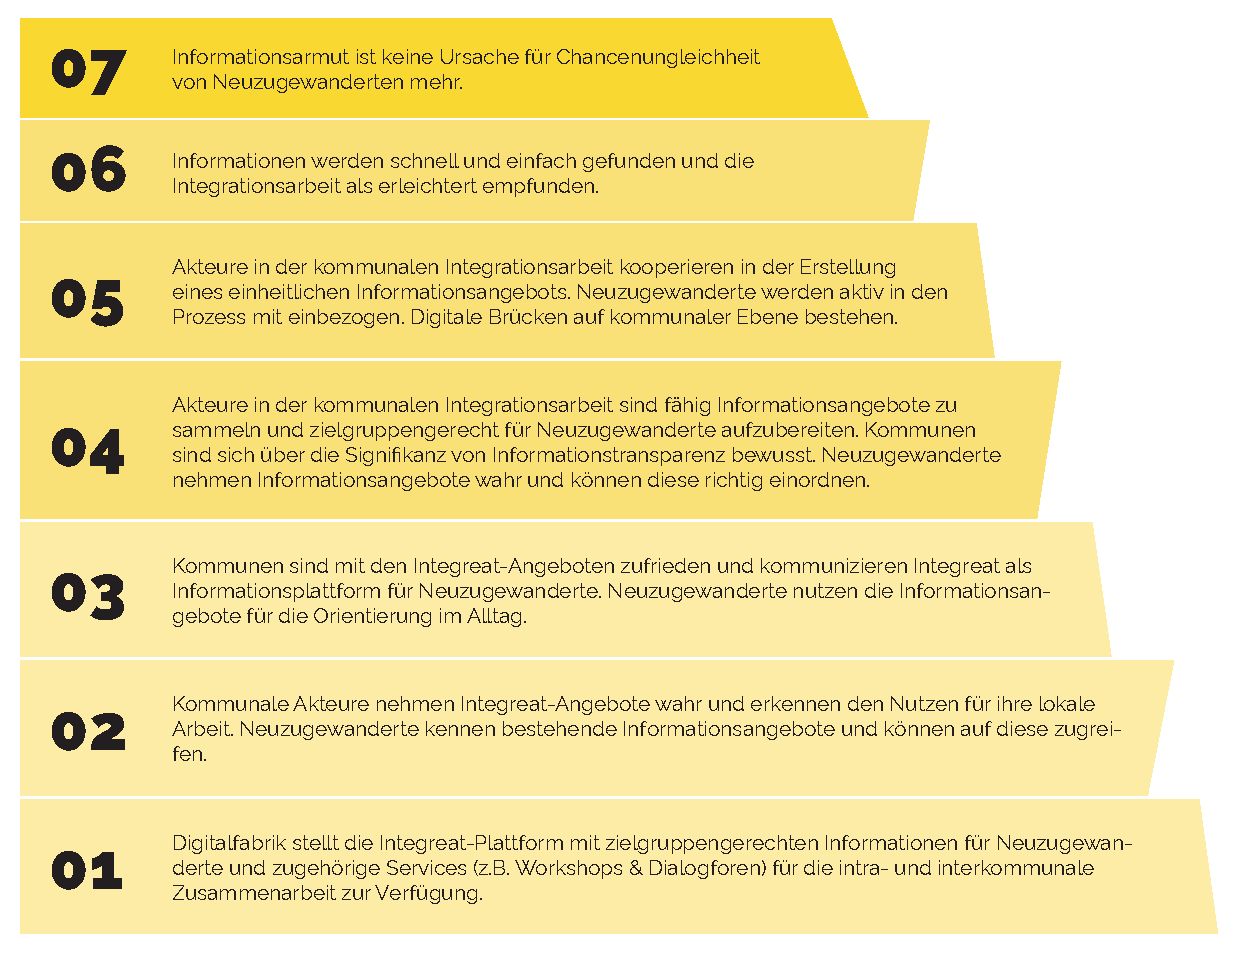
\includegraphics[width=\textwidth]{figure/Treppengrafik.pdf}

\hypertarget{ressourcen-leistungen-und-wirkung-im-jahr-2019-eine-aufstellung}{%
\section{Ressourcen, Leistungen und Wirkung im Jahr 2019 – Eine
Aufstellung}\label{ressourcen-leistungen-und-wirkung-im-jahr-2019-eine-aufstellung}}

\hypertarget{eingesetzte-ressourcen}{%
\subsection{Eingesetzte Ressourcen}\label{eingesetzte-ressourcen}}

Die finanziellen Ressourcen setzen sich im Jahr 2019 aus Personalkosten
in Höhe von 180.000,00 Euro und Sachkosten in Höhe von 45.000,00 Euro
zusammen. Insgesamt wurden im Jahr 2019 somit 225.000,00 Euro zur
Weiterentwicklung der Organisation und der Verbesserung der
Integrationsarbeit deutschlandweit eingesetzt.

Mit einer fluktuierenden Zahl von circa 14 sehr engagierten
Ehrenamtlichen kommen zeitliche Ressourcen von geschätzten 3.500 Stunden
hinzu. Ein großer Teil der ehrenamtlichen Arbeit trug zur technischen
Weiterentwicklung der Integreat-Plattform bei. Der Großteil der
hauptamtlichen Beschäftigten hat sich zunächst ehrenamtlich engagiert
und wurde dann in die Anstellung übernommen.

\hypertarget{erbrachte-leistungen-und-wirkungen-im-integreat-kontext}{%
\subsection{Erbrachte Leistungen und Wirkungen im
Integreat-Kontext}\label{erbrachte-leistungen-und-wirkungen-im-integreat-kontext}}

Aufbauend auf den Leistungen und Wirkungen des letzten Jahres konnte die
Digitalfabrik im Jahr 2019 weitere Fortschritte für die primäre
Zielgruppe der Neuzugewanderten sowie auf kommunaler Ebene erzielen.
Ende 2019 steht Integreat in 57 Städten und Landkreisen in Deutschland
zur Verfügung und hilft dort die Informationsvermittlung an
Neuzugewanderte erfolgreich mitzugestalten. Die Steigerung der Anzahl
der Integreat-Kommunen wirkt sich einerseits auf die Zielgruppe der
Neuzugewanderten aus, da ein größerer Anteil dieser durch Integreat mit
lokalen Informationen versorgt werden kann. Andererseits profitieren
auch die kommunalen Partner der Digitalfabrik von einer stärkeren
Verbreitung der Plattform, da mehr Inhalte und Übersetzungen produziert
werden, die wiederum gemeinschaftlich genutzt werden können und zu
Kosten- und Zeitersparnissen führen.

Durch die Aktivitäten der Digitalfabrik konnten im Jahr 2019 vor allem
Wirkungen auf intrakommunaler Ebene und im interkommunalen Austausch
erreicht werden. Als Indikatoren für diese Wirkungen dienen vor allem
persönliche Berichte und Feedback aus den Kommunen bzw. vom
Integreat-Dialogforum in Bayreuth im November 2019 sowie Beobachtungen
der Mitarbeitenden in der Digitalfabrik. Ein positiver Indikator ist,
dass alle durch die jährliche kommunale Umfrage erreichten
Ansprechpartnerinnen und Ansprechpartner angaben, langfristig mit
Integreat als Teil der lokalen Integrationsarbeit zu planen.

2019 wurde Integreat in 10 Landkreisen und 6 Städten sowie beim
Bayerischen Innenministerium vorgestellt. Workshops im Kontext Integreat
fanden in 7 Landkreisen und 4 Städten u.a. in der Stadt Dortmund, in der
Stadt Sydney und im Landkreis Ludwigsburg vorgestellt. Technische
Schulungen zur Bedienung des Integreat-Systems fanden in insgesamt 13
Landkreisen und 5 Städten statt.

Mit dem Workshop-Angebot bestehend aus einem Auftaktworkshop mit
verschiedenen Akteuren aus dem Integrationsbereich, einer Schulung im
technischen System für die für Integreat zuständigen Personen, einer
Hinführung zum Thema Marketing und der Entwicklung weiterer analoger
Unterstützungsangebote begleitet die Digitalfabrik nicht nur bei
Technologie und Prozessen, sondern trägt auch dazu bei die Menschen vor
Ort stärker in den Gesamtkontext einzubeziehen. In der Zusammenarbeit
mit der bundesweit agierenden Digitalfabrik erkennen kommunale Akteure
Synergiepotentiale und lernen gemeinsam voneinander.

Das Integreat-Dialogforum mit Kommunen und Landkreisen aus ganz
Deutschland hat sich mittlerweile als wichtiger jährlicher Termin für
alle Partnerkommunen im Netzwerk etabliert. Im Jahr 2019 nahmen über 30
Akteure aus 22 Kommunen daran teil. Die Veranstaltung ist beispielhaft
für den Bedarf an interkommunalen Austausch. In diesem Jahr stand
insbesondere der Austausch von Expertenwissen und die Weitergabe von
Best Practices aus der lokalen Arbeit im Mittelpunkt. Impulsvorträge aus
insgesamt vier ausgewählten Kommunen bildeten dabei die Basis für
weitere Diskussionen und das gemeinsame Entwickeln neuer Lösungen.

\hypertarget{leistungen-und-wirkungen-aus-weiteren-projekten}{%
\subsection{Leistungen und Wirkungen aus weiteren
Projekten}\label{leistungen-und-wirkungen-aus-weiteren-projekten}}

Für die Projekte im Augsburger Raum lässt sich beobachten, dass sowohl
die regelmäßig durchgeführten ffIT-Kurse als auch das Internet-Angebot
in den Unterkünften von den Neuzugewanderten, sehr gut angenommen
werden.

Nachdem im Jahr 2018 erfolgreich der erste ffIT-Kurs durchgeführt wurde,
konnte das Kursformat 2019 zwei weitere Male durchgeführt werden. Von
den in allen Jahrgängen zusammengenommenen ca. 70 Teilnehmerinnen und
Teilnehmern konnten rund 50 der Neuzugewanderten den Kurs mit dem Erhalt
eines Zertifikats erfolgreich abschließen und beherrschen nun den
grundlegenden Umgang mit Computern, Smartphones und dem Internet - eine
wichtige Grundlage für die selbstständige Wohnungs- und Jobsuche im
Internet.

Ein weiterer Internetzugang in der Unterkunft im Mühlmahdweg in Augsburg
wurde zum 27.02.2019 erfolgreich in Betrieb genommen. Die Nachfrage ist
in allen durch die Digitalfabrik betreuten Unterkünften hoch und gibt
damit Hinweis auf den starken Bedarf an Internet- und damit
Informationszugang für die dort lebenden Menschen. Durch die Übernahme
des Betriebs in der Schülestraße konnten wir vor allem die dortigen
Ehrenamtlichen im Helferkreis entlasten, da dort monatliche
Vor-Ort-Termine notwendig waren, um Internet-Voucher an die Geflüchteten
zu verkaufen. Durch das organisatorische Konzept der Tür an Tür -
Digitalfabrik, den Verkauf zentral über das in der Innenstadt gelegene
Café Tür an Tür zu organisieren, entfällt die Notwendig für die
Ehrenamtlichen, die sich nun wieder auf andere, relevantere
Unterstützungsleistungen fokussieren können.

\hypertarget{mauxdfnahmen-zur-begleitenden-evaluation-und-qualituxe4tssicherung}{%
\subsection{Maßnahmen zur begleitenden Evaluation und
Qualitätssicherung}\label{mauxdfnahmen-zur-begleitenden-evaluation-und-qualituxe4tssicherung}}

\hypertarget{wissenschaftliche-evaluationen}{%
\subsubsection{Wissenschaftliche
Evaluationen}\label{wissenschaftliche-evaluationen}}

Ein Aspekt, auf den seit der Gründung 2016 viel Wert gelegt wurde ist
die wissenschaftliche Evaluierung der Integreat-Plattform. Seither
wurden zahlreiche Arbeiten verfasst, die sich mit der Rolle und den
Chancen von Informations- und Kommunikationstechnik (ICT) im Kontext der
Integration auseinandersetzen.

Daniel Kehne legte 2018 mit seiner Masterarbeit an der TU München dar,
dass digitale Technologien für Geflüchtete ein entscheidendes Instrument
für die Teilhabe an der Gesellschaft sind, da sie Entscheidungen in der
realen Welt beeinflussen. Aus Interviews mit Menschen mit
Fluchthintergrund konnte mit Hilfe einer qualitativen Analyse abgeleitet
werden, dass die Nutzung von Informationsplattformen dazu führen kann,
dass neben der Beeinflussung von Entscheidungen auch
zwischenmenschlichen Kontakte entstehen, die den Integrationsprozess
weiter begünstigen.

Ebenfalls zu digitalen Technologien als Kommunikationsmittel von
Geflüchteten forschte Hannah Diemer an der Universität Augsburg im
Rahmen ihrer Abschlussarbeit (2018). Die Nutzung von ICTs unterstützt
durch die Weitergabe von Informationen bei der Ankunft in Deutschland.
Durch das Netzwerk, welches sich über soziale Medien aufbauen lässt,
fällt es leichter sich in eine Gesellschaft einzufinden und Freunde oder
Bekannte zu finden und damit das eigene soziale Kapital zu erweitern.
Dies vereinfacht letztendlich ebenfalls den Integrationsprozess. Damit
wurde verdeutlicht, dass im Zeitalter der Digitalisierung und mit dem
Internet die Integration durch die besseren Möglichkeiten zur
Kontaktaufnahme vereinfacht wird. Als Fazit für die Arbeit der
Digitalfabrik kann aus der genannten Forschungsarbeiten gezogen werden,
dass durch unser Auftreten auf dem digitalen Feld ein deutlicher
Mehrwert für die Zielgruppe erreicht werden kann und die Nutzung von
Informationen aus der Integreat-Plattform auf dem Weg in die
Gesellschaft eine Hilfestellung ist.

Einen besonderen Stellenwert im Hinblick auf die wissenschaftliche
Evaluation nimmt zudem die Bachelorarbeit von Janine Rosenbaum an der TU
München ein, die in Zusammenarbeit mit Robert Zepic, Clara Bracklo,
Maximilian Schreieck, Dr. Manuel Wiesche und Prof. Dr. Helmut Krcmar den
Digital Government Excellence Award 2018 auf der 18. European Conference
on Digital Government (ECDG) in Spanien gewann. Die Forschungsarbeit
trägt den Titel “Integreat: An information ecosystem for refugees“. Die
Arbeit zeigt auf welche Gründe es für die Nicht-Nutzung von Mobile
Government-Applikationen gibt. Das Resultat ist, dass nicht das Angebot
selbst verantwortlich dafür ist, wenn es nicht genutzt wird, sondern
hier eher Sprachbarrieren oder die Unbekanntheit des Angebots wirken.
Daraus ziehen wir die Notwendigkeit die Bekanntheit von Integreat zu
steigern und unsere kommunalen Akteure dazu zu befähigen
zielgruppengerechte Marketing-Maßnahmen umzusetzen, um den negativen
Auswirkungen einer digitalen Kluft entgegen zu wirken.

Aus sozialwissenschaftlicher Perspektive wurden ebenfalls Arbeiten
verfasst, die die Rolle der Integreat-Plattform mit einbeziehen. Die
2018 von Georg Meyer eingereichte Masterarbeit an der Pädagogischen
Hochschule Schwäbisch Gmünd behandelt Inhalte, die Neuzugewanderte aus
einer bestimmten Kommune brauchen, um diese schlussendlich in die
Integreat-Plattform einzupflegen. Hieraus lassen sich Bedarfe ableiten,
die auf die benötigten Inhalte für eine erfolgreiche Integration
hinweisen.

Das kooperative Lehrforschungsprojekt “Schon angekommen” des
Fachbereichs Sozialwesen der DHBW Heidenheim und des Landkreises
Heidenheim liefert eine Bestandsaufnahme der Lage von Menschen mit
Migrationserfahrung in Bezug auf die Dimensionen Wohnen, Arbeiten,
Bildung, Sprache, Ehrenamt, soziale Teilhabe und Gesundheit. Bei der
Studie geht es insbesondere um die Einbindung eingewanderter Menschen in
spezifische Teilsysteme der Gesellschaft wie beispielsweise den
Arbeitsmarkt oder das Gesundheitssystem. Sie legt außerdem den Fokus auf
die Angebotswünsche der Menschen mit Migrationserfahrung sowie auf den
Grad der Bekanntheit und die Nutzung bereits bestehender Angebote und
Infokanäle. Die Studie wurde von Oktober 2018 bis August 2019
durchgeführt und beruht auf qualitativen sowie quantitativen
Forschungsmethoden. Für die Integreat-Plattform kann aus den Ergebnissen
des Projekts die Notwendigkeit abgeleitet werden, die bereits erwähnte
Bekanntheitssteigerung von Integreat als wichtiges Ziel in den Blick zu
nehmen.

Die Relevanz der wissenschaftlichen Arbeiten, die im Kontext von
Integreat bereits verfasst wurden, ist enorm. Daher werden
Forschungsarbeiten, die das Wirken der Digitalfabrik thematisieren, auch
zukünftig einen signifikanten Einfluss auf die Unternehmensstrategie
haben.

\hypertarget{weitere-aktivituxe4ten-zur-wirkungsbeobachtung}{%
\subsubsection{Weitere Aktivitäten zur
Wirkungsbeobachtung}\label{weitere-aktivituxe4ten-zur-wirkungsbeobachtung}}

Die Wirkung der unterschiedlichen Projekte der Tür an Tür -
Digitalfabrik soll auch außerhalb der wissenschaftlichen Evaluation
beobachtet werden. Verschiedene Maßnahmen, die hierzu im Kontext des
Integreat-Projektes im Jahr 2019 vorgenommen wurden, sind:

\begin{itemize}
\item

  \textbf{Austausch mit der international agierenden Forschungsstiftung
  J-PAL Europe}

Im Mai 2019 hatte die Digitalfabrik die Möglichkeit in Paris gemeinsam
mit anderen Organisationen und Initiativen aus ganz Europa zu lernen,
wie anhand randomisierter Evaluation die Wirkung von Projekten
nachgewiesen und gemessen werden kann. Der dreitägige Workshop ist Teil
der European Social Inclusion Initiative von J-PAL Europe. Veranstalter
des Workshops war J-PAL Europe, eine Forschungsstiftung, deren Anspruch
es ist basierend auf umfangreichen randomisierten Projektevaluationen
politische Entscheidungsträger zu informieren und zu beraten. Häufig
haben soziale Projekte nicht die finanziellen und personellen Mittel, um
angemessene und aussagekräftige Wirkungsanalysen durchzuführen. In
Zusammenarbeit mit J-PAL werden erfahrene Forscherinnen und Forscher mit
Mitarbeitenden ausgestattet und evaluieren unabhängig die Wirkung
ausgewählter Projekte.

Bei der Auftaktveranstaltung in Paris konnte die Digitalfabrik erste
Eindrücke über Umfang und Vorgehensweise einer solchen
Forschungsinitiative gewinnen. Seither steht die Digitalfabrik im
Austausch mit J-PAL Europe, um Möglichkeiten der Zusammenarbeit zu
identifizieren.

\item  \textbf{Lokal veranstaltete Workshops zur Wirkungsevaluation}

Immer mehr kommunale Partner von Integreat nehmen die Überprüfung der
Wirkung vor Ort als wichtige Aufgabe wahr. Im Jahr 2019 wurden daher in
gleich mehreren Kommunen lokale, selbstorganisierte Workshops zur
Wirkungsevaluation durchgeführt. Der Fokus der Workshops lag dabei u.a.
auf Zielformulierungen, der Entwicklung von lokal überprüfbaren
Wirkungsindizien und der Überprüfung bisheriger Inhalte durch die
Zielgruppe.

\item  \textbf{Versenden automatischer Statistiken}


Integreat ist nach dem Konzept von „Privacy by Design“ und den
Datenschutzanforderungen für Apps des Düsseldorfer Kreises entwickelt
worden und entspricht der EU-Datenschutzgrundverordnung. Anonymisierte
Nutzungsstatistiken d.h. die Anzahl von Online-Abrufen können dennoch
allen Partnerkommunen bereitgestellt werden.

Die Anzahl von Abrufen in den letzten 30 Tagen sind von jeder Kommune
selbst jederzeit im Integreat-System einsehbar. Zudem besteht die
Möglichkeit monatlich automatisch die aktuellen Statistiken per E-Mail
zugesendet zu bekommen.

Monatliche Statistiken ermöglichen es den Entscheidungsträgerinnen und
-trägern einen Eindruck davon zu gewinnen, wie beispielsweise Werbung
für Integreat oder andere Maßnahmen die Nutzung beeinflussen. Diese
Beobachtungen können dabei helfen Integreat zu verbessern und auch viele
Monate nach der Einführung die Wahrnehmung des Angebotes zu evaluieren.
Insbesondere in Verbindung mit gegebenem Feedback sind sie daher ein
wichtiger Bestandteil kommunaler Arbeit. Allerdings müssen die in den
Statistiken angegeben Zahlen immer unter Vorbehalt betrachtet werden, da
beispielsweise Offline-Zugriffe nicht abgebildet werden können. Es
lassen sich also nur Trends und keine Aussagen zur absoluten Nutzung von
Integreat ableiten.

\item  \textbf{Gespräche zur Evaluation kommunaler Entwicklungen}

Ende 2019 setzten beinahe 60 Kommunen deutschlandweit auf Integreat.
Damit wächst das Netzwerk stark an. Viele Kommunen arbeiten seit
mehreren Jahren mit der digitalen Lösung. Ihre Erfahrungen sichtbar zu
machen und zu bündeln ist Ziel von regelmäßigen Telefonaten zum Thema
Wirkung. Die Gespräche finden jährlich zum Jubiläum der Zusammenarbeit
statt und decken Fragen über die Erreichung der vorgenommenen Ziele,
aktuelle Herausforderungen und Wirkungen aus lokaler, kommunaler Sicht
ab.

Folgende Beobachtungen konnten im Jahr 2019 gemacht werden:

Die Systematisierung von Informationen und die Zusammenfassung
bestehender Angebote auf einer zentralen Integrations-Plattform ist mit
der Hauptgrund zur Einführung von Integreat. Weitere Gründe sind die
leichte Anpassbarkeit und Erweiterbarkeit der Zielgruppe, die
Möglichkeit Transparenz für Beraterinnen, Berater und Ehrenamtliche zu
schaffen, die Ergänzung bestehender Angebote sowie der Wunsch ein
Zeichen in der Integrationsarbeit zu setzen.

Integreat wird stets aktualisiert und auch sprachlich erweitert, um den
Bedürfnissen der Nutzerinnen und Nutzer zu entsprechen. Die
Zusammenarbeit mit den Kommunen wird als reibungslos bewertet und
Integreat ist einfach in der Umsetzung. Beraterinnen und Berater,
Neuzugewanderte und Ehrenamtliche kennen und nutzen Integreat, auch wenn
die Bekanntmachung bei Neuzugewanderten und älteren Ehrenamtlichen noch
ausbaufähig ist. Herausforderungen, die nach der Einführung häufig
auftreten, sind die Finanzierung neuer Übersetzungen und die
Aktualisierung von Übersetzungen, die langfristige Anbindung von
Integreat an kommunale Strukturen v.a. bei Stellenwechseln, die
Bekanntmachung von Integreat vor Ort und die Erweiterung der Inhalte für
neue Zielgruppen in der Zusammenarbeit mit unterschiedlichen
Institutionen und Akteuren. Die Zusammenarbeit von Integreat mit den
Kommunen wird als sehr positiv angesehen, besonders die Möglichkeit der
eigenständigen Pflege von Inhalten. Integreat bietet auf kommunaler
Ebene viele Möglichkeiten zur kollaborativen Erstellung von
Informationsinhalten. Die meiste Arbeit wird dabei von zuständiger
Stelle getragen, aber auf Anfragen an andere lokale Akteure z.B. zur
Aktualisierung von bestimmten Seiten oder Kontaktdaten wird positiv
reagiert. Darin zeigt sich das generelle Interesse und die Unterstützung
der Integreat-Plattform auf lokaler Ebene.

\item  \textbf{Kommunale Jahresumfrage}

In der kommunalen Jahresumfrage wird die Digitalfabrik für die
Benutzerfreundlichkeit der Technologie gelobt, die für die
Integreat-Plattform eingesetzt wird. Besonders die Funktionen des
Exports von PDF-Dateien und somit die Möglichkeit, die Inhalte aus
Integreat auch als Broschüre ausdrucken zu können, werden positiv
bewertet. Damit kann der aktuelle Stand der Informationen ausgedruckt
werden und auch diejenigen erreichen, die kein Smartphone besitzen.
Ebenso für gut befunden wird die automatische Bereitstellung von
Statistiken. Integreat legt Wert darauf, problemorientierte
Lösungsansätze zu bieten und den kommunalen Partnern jederzeit bei
Problemen zur Seite zu stehen. Hierfür ist es unerlässlich, einen
schnellen und unkomplizierten Kontakt zwischen dem Integreat-Team und
den lokalen Verwaltungen zu ermöglichen. Dieser Ansatz wird auch von den
zuständigen Stellen in den Kommunen erkannt und positiv wahrgenommen.
Auch die Möglichkeiten des Netzwerkens innerhalb und zwischen kommunalen
Akteuren wird besonders geschätzt. Bei der Funktionalität legen viele
der befragten Kommunen Wert auf eine möglichst barrierearme Nutzbarkeit
von Integreat, um das Angebot allen Menschen zugänglich zu machen.

Die Kommunen wurden ebenfalls nach den Auswirkungen von Integreat
gefragt, die sie 2019 wahrgenommen haben. Die Nutzung von Integreat
erleichtert die Arbeit von Integrationsberaterinnen und
Integrationsberatern. Migrantinnen und Migranten berichten, dass sie
durch die Nutzung von Integreat in der Lage waren, die Kontaktstellen zu
finden, die sie benötigten. Die meisten Kommunen verzichten allerdings
auf eine Bewertung der Auswirkungen von Integreat, weil oft kein
direkter Kontakt mit der Zielgruppe besteht. Alle Kommunen, die an der
Umfrage teilgenommen haben, planen Integreat langfristig als Teil ihrer
Integrationsarbeit ein.
\end{itemize}

\hypertarget{planung-und-ausblick}{%
\section{Planung und Ausblick}\label{planung-und-ausblick}}

\hypertarget{planung-und-ziele}{%
\subsection{Planung und Ziele}\label{planung-und-ziele}}

Nachdem 2019 die Professionalisierung und Ausweitung der Kooperation mit
unseren kommunalen Partnern, der Fokus auf das Thema der
Arbeitsmigration, die Bekanntmachung von Integreat außerhalb
Deutschlands und die Entwicklung von Innovationsprozessen als Ziele
gesetzt wurden, steht das Jahr 2020 im Zeichen der nachhaltigen
Entwicklung in Finanzierung, Technologie, Strategie und
Organisationsstruktur und der Förderung von Diversität.

\begin{enumerate}
\def\labelenumi{\arabic{enumi}.}
\item \textbf{Nachhaltigkeit als Grundlage}

Finanzielle Unabhängigkeit und Sicherheit sind zur Entwicklung von
nachhaltigen, langfristigen und damit wirkungsvollen Projekte
unabdingbar. Die Digitalfabrik ist eine gemeinnützige GmbH und damit
nicht auf finanziellen Profit, sondern auf die Verbesserung
gesellschaftlicher Bedingungen ausgerichtet. Anders als andere soziale
Projekte, die beispielsweise von Spendengeldern finanziert werden,
ermöglichen projektbezogene Geschäftsmodelle der Digitalfabrik die
selbstbestimmte Gestaltung von Prozessen sowie eine hohe Sicherheit
durch zeitliche Planbarkeit über Förderzeiträume hinweg. Bereits 2019
wurde damit begonnen Projekteinnahmen zu stabilisieren und eine sichere
Grundlage für neue Projekte zu schaffen. Diese Unternehmungen sollen
2020 weitergeführt werden, um langfristig finanziell unabhängig agieren
zu können.

Auch auf der Ebene der Organisationsentwicklung sollen 2020 nachhaltige
Strukturen etabliert werden. Seit der Gründung der Digitalfabrik 2016
ist das Team zunächst im Kontext der Integreat-Plattform und mit neuen
Projekten auch darüber hinaus gewachsen. Strukturen der Kommunikation
und Zusammenarbeit entwickelten sich organisch mit neuen Bedarfen und
Aufgaben. Durch die Professionalisierung der Digitalfabrik in den
letzten Jahren und dem wachsenden Team wird der Bedarf nach klaren
Strukturen und Transparenz in der internen Kommunikation immer
deutlicher, so dass sich auch neue Mitarbeiterinnen und Mitarbeiter
schnell zurechtfinden. Durch eine übersichtliche Online-Dokumentation
(unter: wiki.integreat-app.de) und den Ausbau von Teamstrukturen wurden
bereits erste Schritte getan. Des Weiteren sollen zeitintensive
Aufgaben, insbesondere die kommunale Betreuung, auf mehrere Schultern
verteilt werden, um so unabhängig von einzelnen Personen langfristig
handlungsfähig zu sein.

Für das Projekt Integreat steht im Jahr 2020 zusätzlich die technische
Nachhaltigkeit im Fokus. Die neue Integreat-Plattform wird technologisch
auf ein neues Fundament (React) gesetzt. Die Vorteile: Moderne
Architektur, bessere Ladezeiten und vor allem verkürzte
Entwicklungszyklen, d.h. neue Funktionen können schneller entwickelt
werden. Auch das Inhaltsverwaltungssystem der Integreat-Plattform, das
von Integrationsakteuren in ganz Deutschland genutzt wird, um Inhalte zu
erstellen und zu pflegen, soll mit einer neuen Technologie
nutzerfreundlicher und intuitiver gestaltet werden. So kann die
benötigte technische Unterstützung durch unsere Beraterinnen und Berater
minimiert werden und die Integreat-Technologie ist leichter für andere
Kontexte adaptierbar.

\item \textbf{Diversität im Team}

Als Sozialunternehmen stellt für die Digitalfabrik nicht nur die
Wirksamkeit der einzelnen Projekte eine wichtige Komponente dar, sondern
auch die positive Gestaltung von internen Strukturen. In der Akquise von
neuen Mitarbeitenden sowie Ehrenamtlichen soll die
Geschlechterdiversität und die Interkulturalität besonders gefördert
werden. Die durch das Teilzeitmodell geprägte Unternehmenskultur der
Digitalfabrik, die flexiblen Arbeitszeiten und die Möglichkeiten zur
Arbeit im Homeoffice machen dies in besonderem Maße möglich. Nur so kann
die Entwicklung von sozialen Projekten im digitalen Bereich inklusiv
gestaltet werden.

\end{enumerate}

\hypertarget{chancen-und-risiken}{%
\subsection{Chancen und Risiken}\label{chancen-und-risiken}}

Wie bereits im letzten Wirkungsbericht vorhergesehen hat sich in der
kommunalen Integrationsarbeit eine Bewegung in der Zielgruppe von
Integreat vollzogen und Integration wird vermehrt im Kontext von
EU-Migration betrachtet. Integration von Geflüchteten steht nicht mehr
im gleichen Umfang im Mittelpunkt der Aufmerksamkeit wie noch vor
einigen Jahren und in diesem Sinne sind weniger Fördergelder verfügbar
oder Förderprogramme laufen aus. Dies beeinflusst sowohl die direkte
Finanzierbarkeit von Integreat für Kommunen als auch die Bereitstellung
weiterer langfristiger Ressourcen (z.B. hauptamtlicher Stellen zur
inhaltlichen Pflege) und die Aktualisierung bzw. Erweiterung von
Übersetzungen.

Das im März 2020 in Kraft getretene Fachkräfteeinwanderungsgesetz
bedingt diese Entwicklung zusätzlich. Die Einreise und der Erhalt eines
Aufenthaltstitels werden deutlich erleichtert. Allerdings herrscht ein
großer Informations- und Unterstützungsbedarf bei der Rekrutierung
ausländischer Fachkräfte. Für eine erfolgreiche Sicherung und
Integration von Arbeitskräften aus dem Ausland spielt die Zusammenarbeit
aus den Akteuren der Wirtschaft und des Arbeitsmarktes mit den Akteuren
der Integrationsarbeit eine wichtige Rolle. Die Digitalfabrik beobachtet
diese Entwicklungen aktiv und entwickelt bestehende und neue Projekte
dementsprechend.

Die zu Beginn des Jahres 2020 eingetretene gesellschaftliche
Ausnahmesituation durch die Verbreitung des Coronavirus (COVID-19)
verdeutlicht die Relevanz von schneller, einfacher und verständlicher
Informationsvermittlung an alle Menschen. Der Bedarf an digitalen
Lösungen kann in Zukunft zu einer steigenden Nachfrage nach
Unterstützungsangeboten wie Integreat beitragen.

\hypertarget{organisationsstruktur-und-team}{%
\section{Organisationsstruktur und
Team}\label{organisationsstruktur-und-team}}

\hypertarget{organisationsstruktur}{%
\subsection{Organisationsstruktur}\label{organisationsstruktur}}

Auch in der Organisationsstruktur der Digitalfabrik nimmt das Projekt
Integreat eine besondere Rolle ein. Während die Digitalfabrik
hauptamtliche Mitarbeiterinnen und Mitarbeiter für die Arbeit an
Integreat sowie an anderen Projekten beschäftigt, engagieren sich im
Integreat-Projekt (wie auch im WLAN-Projekt in Augsburg) auch weiterhin
viele Ehrenamtliche.

Zwischen hauptamtlichen und ehrenamtlichen Mitarbeitenden bestehen
teilweise große Unterschiede in dem Umfang ihrer Arbeit für das
Integreat-Projekt. Um zu vermeiden, dass Ehrenamtliche abgehängt werden
und ihren Beitrag zum Projekt nicht mehr leisten können, sind die
bezahlten Wochenstunden von Hauptamtlichen auf 20 Stunden pro Projekt
gedeckelt. Die verschiedenen Arbeitsbereiche werden je nach Bedarf von
größeren oder kleineren Teams abgedeckt.

Ein großer Teil der Mitarbeitenden absolviert parallel ein Studium,
sodass unsere Organisation auf individuelle Arbeitszeitmodelle und
dynamische Anforderungen an die Projektkoordination reagieren können
muss. Personen, die schon länger Teil des Teams und Projekts sind,
kümmern sich um das Einarbeiten von neuen Mitarbeitenden. Hauptamtliche
Angestellte stehen in den einzelnen Arbeitsbereichen als Konstante und
Ansprechpersonen für Unklarheiten und operative Herausforderungen mit
zeitlichen Fristen zur Verfügung. Auf den vierteljährlich stattfindenden
Integreat-Konferenzen der Digitalfabrik treffen sich alle Mitarbeitenden
physisch für zwei Tage und tauschen sich über aktuelle Aufgaben,
Herausforderungen, Bedarfe und Entwicklungen aus und definieren
gemeinsam strategische Meilensteine und Ziele. So werden auch in einer
virtuellen Organisation, deren Mitglieder sich über verschiedene Teile
Deutschlands erstrecken, gute Zusammenarbeit und eine gemeinsame
Organisationskultur erhalten.

\hypertarget{kooperationen-partnerschaften-und-netzwerke}{%
\subsection{Kooperationen, Partnerschaften und
Netzwerke}\label{kooperationen-partnerschaften-und-netzwerke}}

Historisch bedingt spielen die Gesellschafter der Digitalfabrik auch im
Bereich der Partnerschaften, Kooperationen und Netzwerke eine zentrale
Rolle. Über den Hauptgesellschafter, den Tür an Tür e.V., besteht eine
starke Vernetzung mit Integrationsprojekten in Augsburg. Der Verein
existiert seit 1992 in Augsburg und setzt sich seitdem in regionalen
Projekten für die Chancen und Rechte von Geflüchteten, Migrantinnen und
Migranten ein.

Die übrigen Gesellschafter, ihres Zeichens Mitarbeitende der TU München,
bringen nicht nur ihre Expertise im Bereich der Softwarearchitektur ein,
sondern öffnen auch regelmäßig ihre Kontakte in die nationale
E-Government-Szene und zu anderen Forschungseinrichtungen. Darüber
hinaus ist der Lehrstuhl für Wirtschaftsinformatik nach wie vor
Ausrichter der vierteljährlichen Konferenzen des Integreat-Projekts,
Forschungspartner für diverse Problemstellungen der Digitalfabrik und
Betreuer von Abschlussarbeiten im Kontext der Tätigkeiten der
Digitalfabrik. Bei Gelegenheit wird die Digitalfabrik in
Lehrveranstaltungen und Seminaren als Praxispartner einbezogen.

Die im Laufe des Jahres 2017 geschlossenen Partnerschaften mit der
Vereinigung der Bayerischen Wirtschaft e.V. für die Praktikumsbörse
„sprungbrett into work“, und mit der Handwerkskammer für den
„Lehrstellenradar“ bestehen auch weiterhin. Die genannten Plattformen
konnten über Schnittstellen in die Integreat-Plattform integriert
werden, ohne dass Ressourcen für neue Entwicklungen von der
Digitalfabrik aufgewendet werden mussten. Die Kooperationen steigern die
Wirkung auf allen Seiten.

Die Zusammenarbeit mit dem Übersetzungsbüro tolingo wurde Ende des
Jahres 2019 um erste Aufträge in Kooperation mit dem Münchner
Übersetzungsdienstleister linguarum ergänzt. Ein Rahmenvertrag mit
linguarum soll Anfang 2020 in Kraft treten. Der stark gewachsene
Übersetzungsspeicher, eine Datenbank mit allen bereits bestehenden
Übersetzungen und Texten aus allen Kommunen, auf den beide
Übersetzungsbüros zugreifen können, verhilft den Kommunen und Kreisen zu
deutlichen Einsparungen beim Einkauf der Übersetzungsdienstleistungen.

Die Digitalfabrik war Teil der „Teilhabe Wirkungsschmiede“ des „Programm
Engagement mit Perspektive“ von Ashoka Deutschland. Gemeinsam mit
anderen Sozialunternehmen wurde insbesondere die Wirkungsausrichtung der
jeweiligen Aktivitäten auf den Prüfstand gestellt. Die grundlegende
Ausrichtung der Strategien der Digitalfabrik sind von diesem Austausch
geprägt. Als Alumni des Programms ist die Digitalfabrik zudem Teil eines
großen Netzwerks von Unternehmungen mit denselben Werten und Visionen.

\hypertarget{organisationsprofil}{%
\section{Organisationsprofil}\label{organisationsprofil}}

\hypertarget{allgemeine-angaben}{%
\subsection{Allgemeine Angaben}\label{allgemeine-angaben}}
\noindent\begin{adjustwidth}{-1cm}{-1cm}
  \begin{tabularx}{\textwidth+2cm}{p{5cm}X}
  \toprule
  Name & Tür an Tür – Digital Factory gGmbH\tabularnewline
  \midrule
  Sitz der Organisation gemäß Satzung & Augsburg\tabularnewline
  \midrule
  Gründung & 22.06.2016\tabularnewline
  \midrule
  Rechtsform & gemeinnützige GmbH\tabularnewline
  \midrule
  \begin{minipage}[t]{0.47\columnwidth}\raggedright
  Kontaktdaten\strut
  \end{minipage} & \begin{minipage}[t]{\columnwidth}
  Wertachstr. 29
  
  86153 Augsburg
  
  \href{mailto:digitalfactory@tuerantuer.de}{\url{digitalfactory@tuerantuer.de}}
  
  \url{https://tuerantuer.de/digitalfabrik/}
  \end{minipage}\tabularnewline
  \midrule
  Link zur Satzung (URL) & \url{https://tuerantuer.de/wp-content/uploads/2017/05/Gesellschaftsvertrag\_TATDF\_final.pdf}\tabularnewline
  \midrule
  Registeramt & Finanzamt Augsburg-Stadt\tabularnewline
  Registernummer & HRB30759\tabularnewline
  Datum der Eintragung & 27.06.2016\tabularnewline
  \midrule
  Angabe über die Gemeinnützigkeit gemäß §52 Abgabenordnung. Datum des
Feststellungsbescheids, Ausstellendes Finanzamt, Erklärung des
gemeinnützigen Zwecks & Gemeinnützigkeit gemäß §52 Abgabenordnung festgestellt am 29.08.2019 vom
  Finanzamt Augsburg-Stadt 
  (1) Gegenstand des Unternehmens ist a. die Förderung der Hilfe für
  politisch, rassisch oder religiös Verfolgte, für Flüchtlinge,
  Vertriebene, Aussiedler, Spätaussiedler, Kriegsopfer,
  Kriegshinterbliebene, Kriegsbeschädigte und Kriegsgefangene,
  Zivilbeschädigte und Behinderte sowie Hilfe für Opfer von Straftaten;
  
  Förderung des Andenkens an Verfolgte, Kriegs- und Katastrophenopfer;
  Förderung des Suchdienstes für Vermisste; b. die Förderung des
  Wohlfahrtswesens, insbesondere der Zwecke der amtlich anerkannten
  Verbände der freien Wohlfahrtspflege (§ 23 der Umsatzsteuer
  Durchführungsverordnung), ihrer Unterverbände und ihrer angeschlossenen
  Einrichtungen und Anstalten; c. die Förderung der
  Entwicklungszusammenarbeit; d. die Förderung des bürgerschaftlichen
  Engagements zugunsten gemeinnütziger, mildtätiger und kirchlicher
  Zwecke. e. die Förderung von Wissenschaft und Forschung; f. die
  Förderung der Erziehung, Volks- und Berufsbildung einschließlich der
  Studentenhilfe\tabularnewline
  \midrule
  Anzahl MitarbeiterInnen & 28 \tabularnewline
  davon hauptamtlich & 12 \tabularnewline
  davon Honorarkräfte & 2 \tabularnewline
  davon ehrenamtlich & 14 \tabularnewline
  \bottomrule
  \end{tabularx}
  \end{adjustwidth}

\hypertarget{governance-der-organisation}{%
\subsection{Governance der
Organisation}\label{governance-der-organisation}}

\hypertarget{leitungs--und-geschuxe4ftsfuxfchrungsorgan}{%
\subsubsection{Leitungs- und
Geschäftsführungsorgan}\label{leitungs--und-geschuxe4ftsfuxfchrungsorgan}}

Die Tür an Tür - Digitalfabrik wird von Daniel Kehne und Fritjof Knier
als gleichberechtigte Geschäftsführer nach außen vertreten. Beide
Geschäftsführer sind alleinvertretungsberechtigt und üben diese Aufgabe
ehrenamtlich aus. Daniel Kehne wurde 1990 im westfälischen Ahlen
geboren. Nach dem Abitur auf einem technischen Gymnasium absolvierte er
ein duales Studium in der IT-Sparte der Siemens AG. Ab 2012 arbeitete er
als Prozessberater beim französischen IT-Konzern Atos. Von 2014 bis 2018
studierte er an der Universität Augsburg und TU München Finance \&
Information Management und schloss dieses im März 2018 erfolgreich ab.
Im April 2015 rief er das Projekt Integreat ins Leben und übernahm mit
der Gründung der Digitalfabrik gemeinsam mit Fritjof Knier die Aufgabe
als Geschäftsführer.

Fritjof Knier wurde 1990 in Heide geboren. Nach seinem dualen Studium
der Betriebswirtschaftslehre an der Europäischen Fachhochschule
Rhein/Erft, der Ausbildung zum Industriekaufmann bei der Neuman \& Esser
Group und einem Praktikum in der Unternehmensberatung INVERTO, begann er
2014 das Studium Finance \& Information Management an der Universität
Augsburg und der Technischen Universität München und schloss dieses im
September 2017 erfolgreich ab. Im November 2015 stieß Fritjof Knier als
Projektmanager zum Projekt Integreat und übernahm mit der Gründung der
Tür an Tür - Digitalfabrik einen der beiden Geschäftsführerposten.
Gemeinsam leiten Daniel Kehne und Fritjof Knier die Tür an Tür -
Digitalfabrik. Daniel Kehne übernimmt dabei die Rolle des Sprechers und
verantwortet jegliche Netzwerktätigkeiten und strategische
Partnerschaften. Fritjof Knier verantwortet die Bereiche Finanzen,
Personal und Organisation.

\hypertarget{aufsichtsorgan}{%
\subsubsection{Aufsichtsorgan}\label{aufsichtsorgan}}

Die Gesellschafterversammlung stellt den Jahresabschluss fest, trifft
Beschlüsse zur Ergebnisverwendung und entlastet die Geschäftsführung.
Die Gesellschafterversammlung tagt einmal jährlich und setzt sich
zusammen aus dem Vorstand des Tür an Tür e.V., namentlich in 2017
Christine von Gropper, Thomas Körner-Wilsdorf, Matthias Schopf-Emrich,
Helmut Schwering und Dr. Stefan Wagner sowie vom Lehrstuhl für
Wirtschaftsinformatik der Technischen Universität München Prof. Dr.
Helmut Krcmar und Maximilian Schreieck, sowie von Dr. Manuel Wiesche,
der als Junior-Professor an der Technischen Universität Dortmund lehrt.

\hypertarget{interessenskonflikte}{%
\subsubsection{Interessenskonflikte}\label{interessenskonflikte}}

Es existieren keine personellen Überschneidungen von Leitungs- und
Aufsichtsorgan. Die Geschäftsführer sind keine Anteilseigner. Die
Gesellschafter bringen sich, auf ausdrücklichen Wunsch der
Geschäftsleitung, in unregelmäßigen Abständen mit inhaltlichen
Vorschlägen in das Alltagsgeschäft ein.

\hypertarget{internes-kontrollsystem}{%
\subsubsection{Internes
Kontrollsystem}\label{internes-kontrollsystem}}

Fritjof Knier ist zuständig für das monatliche Controlling. Ausgaben
werden von beiden Geschäftsführern gemeinsam entschieden, Rechnungen
ebenfalls von beiden geprüft.

\hypertarget{eigentuxfcmerstruktur-mitgliedschaften-und-verbundene-organisationen}{%
\subsection{Eigentümerstruktur, Mitgliedschaften und verbundene
Organisationen}\label{eigentuxfcmerstruktur-mitgliedschaften-und-verbundene-organisationen}}

\hypertarget{eigentuxfcmerstruktur}{%
\subsubsection{Eigentümerstruktur}\label{eigentuxfcmerstruktur}}

Das Stammkapital der Tür an Tür – Digitalfabrik beträgt 25.000 Euro.
Hauptgesellschafter der Tür an Tür – Digitalfabrik ist der Tür an Tür –
miteinander wohnen und leben e.V., der 70\% der Anteile hält. Nach außen
vertreten wird der Verein durch den fünfköpfigen Vorstand. Die übrigen
30\% halten Einzelpersonen, die bereits zu Beginn des Projekts Integreat
beteiligt waren und zum Zeitpunkt der Gründung alle dem Lehrstuhl für
Wirtschaftsinformatik der Technischen Universität München angehörten.
Dies ist der Lehrstuhlinhaber Prof. Dr. Helmut Krcmar (14\% der
Anteile), Prof. Dr. Manuel Wiesche (8\%) sowie Dr. Maximilian Schreieck
(8\%).

\hypertarget{mitgliedschaften-in-anderen-organisationen}{%
\subsubsection{Mitgliedschaften in anderen
Organisationen}\label{mitgliedschaften-in-anderen-organisationen}}

Die Digitalfabrik ist seit der Gründung des Social Entrepreneurship
Netzwerk Deutschland e.V. (SEND) am 24.05.2017 Mitglied in diesem. Die
Digitalfabrik ist zudem seit Juli 2017 Mitglied im NETZWERK Unternehmen
integrieren Flüchtlinge (NUiF) einem Servicenetzwerk des Deutscher
Industrie- und Handelskammertags, um gemeinsam mit Unternehmen und
Arbeitgeberexpertinnen und -experten Best Practices und Ideen rund um
die Beschäftigung von geflüchteten Menschen auszutauschen.

\hypertarget{verbundene-organisationen}{%
\subsubsection{Verbundene
Organisationen}\label{verbundene-organisationen}}

Die Tür an Tür – Digitalfabrik hat keine Verbindungen mit
Organisationen, die über eine Mitgliedschaft hinausgehen. Die
Digitalfabrik hält keine Anteile anderer Organisationen.

\hypertarget{umwelt--und-sozialprofil}{%
\subsection{Umwelt- und
Sozialprofil}\label{umwelt--und-sozialprofil}}

\begin{itemize}
\item
 
  Die Digitalfabrik vergibt Arbeitsverträge mit einer Mindestanzahl zu
  nehmender Urlaubstage. Ermöglicht wird so eine größtmögliche
  Flexibilität der Mitarbeitenden und höchstmögliche Selbstbestimmung
  durch die Arbeitnehmerinnen und Arbeitnehmer.

\item

  Arbeitsorte können von den Mitarbeitenden frei gewählt werden und
  werden von der Digitalfabrik bestmöglich, im Rahmen der zur Verfügung
  stehenden Möglichkeiten, ausgestattet.
  
\item

  Die Arbeitszeit ist von den Mitarbeitenden vollständig frei zu wählen.
  Regelmäßige Abstimmungsgespräche sichern gleichzeitig eine
  bestmögliche Vernetzung der Belegschaft.

\item
  
  Reisen der Digitalfabrik werden in aller Regel mit dem öffentlichen
  Nah- und Fernverkehr (2. Klasse) unternommen. Nur in Ausnahmefällen
  wird auf PKW und Flugzeug zurückgegriffen.
  
\item
 
  Die Belegschaft und die Anteilseigner werden durch monatliche
  Zusammenfassungen durch die Geschäftsführer über alle relevanten
  Geschehnisse informiert.
 
\item
  
  Richtungsweisende strategische Entscheidungen werden in den einzelnen
  Projekten der Digitalfabrik von haupt- und ehrenamtlichen
  Mitarbeitenden gemeinsam getroffen.
 
\item
 
  Hauptamtliche Mitarbeitende und zeitlich stark engagierte
  Ehrenamtliche erhalten separate fachliche und
  persönliche/organisatorische Mentoren (ggf. auch projektunabhängig) an
  die Seite gestellt.

\end{itemize}

\hypertarget{finanz--und-rechnungslegung}{%
\section{Finanz- und
Rechnungslegung}\label{finanz--und-rechnungslegung}}

\hypertarget{buchfuxfchrung-und-rechnungslegung}{%
\subsection{Buchführung und
Rechnungslegung}\label{buchfuxfchrung-und-rechnungslegung}}

Die Buchführung der Tür an Tür - Digitalfabrik gGmbH wird von der
Steuerberaterin Evelyn Zuber, Augsburg (extern) durchgeführt, die
ebenfalls die Erstellung des Jahresabschlusses und der Bilanz übernimmt.
Der Geschäftsabschluss für das Jahr 2019 wird erst zum Ende dieses
Jahres erstellt, sodass wir hier lediglich eine Schätzung der Einnahmen
und Ausgaben für das Jahr 2019 vornehmen werden.

\hypertarget{einnahmen-und-ausgaben}{%
\subsection{Einnahmen und Ausgaben}\label{einnahmen-und-ausgaben}}

\begin{tabularx}{\textwidth}{Xp{2cm}}
  \toprule
  \textbf{Währung, Einheit} & \textbf{Euro, \euro}\tabularnewline
  \midrule
  \textbf{Einnahmen} &\tabularnewline
  1. Erlöse & 126.997,09\tabularnewline
  Davon aus öffentlichen Aufträgen & 0,00\tabularnewline
  2. Zuwendungen & 0,00\tabularnewline
  Davon aus öffentlicher Hand (Zuschüsse) & 0,00\tabularnewline
  3. Beiträge & 0,00\tabularnewline
  4. Sonstige Einnahmen (Preisgelder, Spenden) & 788,89\tabularnewline
  \textbf{Summe Einnahmen} & 127.785,98\tabularnewline
  \midrule
  \textbf{Ausgaben (wenn Sie weniger als 500.000 Euro Gesamteinnahmen
  haben)} &\tabularnewline
  1. Personalkosten & 180.698,07\tabularnewline
  2. Sachkosten & 44.579,35\tabularnewline
  3. Finanzierungskosten & 0,00\tabularnewline
  4. Steuern & 0,00\tabularnewline
  5. Sonstige Ausgaben & 0,00\tabularnewline
  \textbf{Summe Ausgaben} & 225.277,42\tabularnewline
  \midrule
  \textbf{Jahresergebnis (Einnahmen abzgl. Ausgaben)} &
  -97.441,44\tabularnewline
  \bottomrule
  \end{tabularx}

\hypertarget{finanzielle-situation-und-planung}{%
\subsection{Finanzielle Situation und
Planung}\label{finanzielle-situation-und-planung}}

Ein langfristig ausgegebenes Ziel war das Erreichen einer größeren
Unabhängigkeit von Fördergeldern, wobei das Jahr 2019 einen wichtigen
Meilenstein beschreibt. Erstmals seit der Gründung erhielt die
Digitalfabrik im Jahr 2019 keine direkten Fördergelder mehr. Lediglich
über das Welcome Programm des Deutsch Akademischen Auslandsdienst (DAAD)
konnten weiterhin studentische Hilfskräfte, angestellt an
Partnerhochschulen, am Projekt Integreat mitwirken.

Die Erlöse konnten im Vergleich zum Vorjahr (61.000,00 Euro im Jahr
2018) verdoppelt werden und somit auch die nun fehlenden öffentlichen
Fördergelder (55.000,00 Euro im Jahr 2018) ausgleichen werden. Der
Anteil eigener Umsätze an den Gesamteinnahmen - schließt man die
Förderung des DAAD mit ein - lag im Jahr 2019 bei 80 \%.

Der Anteil der Einnahmen durch das umsatzstärkste und kostenintensivste
Projekt der Digitalfabrik - Integreat - ist im Jahr 2019 noch einmal
gestiegen und macht mit etwa 122.000,00 Euro über 95 \% aller Einnahmen
aus. Eine höhere Diversifikation bei Projekten wäre in Zukunft zwar
wünschenswert, da es sich hier aber um Einnahmen aus
Kooperationsverträgen mit 49 Kommunen handelt, sind die Einnahmen der
Digitalfabrik bereits in hohem Maße diversifiziert.

Für eine größere Projektvielfalt wurden im Jahr 2019 zwei
Teilzeitstellen in der “Denkfabrik” geschaffen, um neue Projektideen zu
evaluieren. Die sichtbaren Potenziale dieser Arbeit waren zum Jahresende
als so erfolgsversprechend einzuschätzen, dass die “Denkfabrik”
weitergeführt werden soll.

Im Jahr 2019 wurde zwei weitere Gemeinschaftsunterkünfte in Augsburg mit
notwendiger WLAN-Infrastruktur und einem entsprechenden zentralen
Internetzugang ausgestattet. So erhalten Bewohnerinnen und Bewohner in
mittlerweile 5 großen Unterkünften für einen monatlichen Beitrag von
fünf Euro einen Internetzugang mit angemessener und ausreichender
Geschwindigkeit. Einnahmen in Höhe von 4.500,00 Euro standen Ausgaben in
Höhe von 2.000,00 Euro gegenüber.

Der durchaus nennenswerte Verlust in Höhe von 97.000,00 Euro ist als
eingeplant zu bewerten, da das Preisgeld der Google.org Impact Challenge
aus dem Jahr 2018 in Höhe von 250.000,00 Euro dafür eingesetzt wurde,
die Digitalfabrik mit einem stärkeren personellen Fundament
auszustatten, um insbesondere das Wachstumspotential von Integreat zu
stärken. Wie die Umsätze zeigen, ist dies der Digitalfabrik auch
gelungen.

\hypertarget{mittelherkunft-fuxf6rdergelder}{%
\subsubsection{Mittelherkunft
Fördergelder}\label{mittelherkunft-fuxf6rdergelder}}

Wie bereits erwähnt, erhält die Digitalfabrik für das Projekt Integreat
eine personelle Förderung durch den Deutsch Akademischen Austauschdienst
(DAAD) in Form von drei Stellen für Studentische Hilfskräfte (SHK) über
das Programm „Welcome – Studierende engagieren sich für Flüchtlinge“.
Die Partneruniversität ist die die Technische Universität München, über
die 3 und zeitweise 4 Studierende angestellt wurden. Das Gesamtvolumen
dieser Förderung betrug im Jahr 2019 etwa 30.000 Euro.

\hypertarget{sonstige-einnahmen}{%
\subsubsection{Sonstige Einnahmen}\label{sonstige-einnahmen}}

Die Digitalfabrik erhielt im Jahr 2019 keine nennenswerten sonstigen
Einnahmen.

\hypertarget{ausblick}{%
\subsubsection{Ausblick}\label{ausblick}}

Das Jahr 2019 war ein wichtiger Schritt, um die Digitalfabrik auf
nachhaltiges finanzielles Fundament zu stellen, das sich stärker aus
erzielten Umsätzen speist und so die Unsicherheiten aus der
Förderungslandschaft geringhält. Die Nachfrage und Umsatzentwicklung bei
Integreat im Jahr 2019 ermutigt zu der Annahme, dass die erzielten
Einnahmen schon mittelfristig kostendeckend sein werden. Ein Ausbau der
hauptamtlichen Ressourcen sowohl in der kommunalen Betreuung als auch
der technischen Entwicklung werden für das Jahr 2020 zusätzlich ins Auge
gefasst, sollte sich die erhöhte Nachfrage bei Integreat verstetigen.

Den Aktivitäten der Denkfabrik folgten im Jahr 2019 noch keine konkreten
Projekte oder Lösungen, allerdings wurden wertvolle Grundsteine für
solche gelegt, die im Jahr 2020 positiv zur nachhaltigen Finanzierung
der Digitalfabrik beitragen werden.

Da das Preisgeld der Google.org Impact Challenge im Jahr 2018 in voller
Höhe ausgezahlt wurde, aber bei Integreat über 2 Jahre verteilt in den
Aufbau einer nachhaltigen personellen Struktur investiert wird, wird
auch im kommenden Jahr noch mit einem jährlichen Verlust gerechnet
werden, der aber um die Hälfte geringer ausfallen sollte.

\end{document}
